\documentclass{article}
\usepackage[utf8]{vietnam}
\usepackage{graphicx}
\usepackage{amsmath}
\usepackage{amssymb}
\usepackage{hyperref}
\usepackage{caption}
\usepackage{subcaption}
\usepackage[a4paper, total={6in, 8in}]{geometry}

\title{A gentle introduction to Machine Learning and some simple Neural Network Models \\ \Large Report Lab Week 9-10-11-12-13}
\author{Ngọc Thuận - IPSAL LAB}
\date{March 2023}

\begin{document}

\maketitle
\begin{abstract}
Trong các bài trước chúng ta đã đi qua một loạt các vấn đề mà Thị giác máy tính cổ điển quan tâm, với những phương pháp thô sơ dựa trên các mô hình xử lí tín hiệu cổ điển. Trong bài này chúng ta sẽ lướt qua vấn đề đang là hạt nhân của Thị giác máy tính nói riêng và rất nhiều các lĩnh vực khác nói chung đang hướng đến và đã được áp dụng đến bởi những thành tựu đột phá của nó: Học máy (Machine Learning). Những vấn đề cơ bản sẽ được đề cập là phương pháp tối ưu Gradient Descent và một số mô hình mạng neural cơ bản.   
\end{abstract}
\tableofcontents
\newpage

\section{What is Machine Learning?}
Định nghĩa kinh điển cho một thuật toán Machine Learning như sau: "A
computer program is said to learn from experience E with respect to some tasks
T and performance measure P, if its performance at tasks in T, as measured by
P, improves with experience E.".
\\\\
Tạm dịch: \textit{Một chương trình máy tính được gọi là "học tập" từ kinh nghiệm E để hoàn thành nhiệm vụ T với hiệu quả đo bằng phép đánh giá P, nếu hiệu quả của nó khi thực hiệu nhiệm vụ T, khi được đánh giá bởi P, cải thiện theo kinh nghiệm E.}
\\\\
Nhìn một cách đơn giản hơn có thể cho rằng một mô hình học máy giống như một mô hình thống kê toán học. 
\begin{enumerate}
    \item Thu thập dữ liệu (thu thập mẫu)
    \item Xây dựng mô hình (xác định mô hình thống kê)
    \item Xác định ra các tham số mô hình (ước lượng)
    \item Giải các bài toán tùy theo yêu cầu thực tế
\end{enumerate}
Cách nhìn trên có lẽ là gần gũi hơn, cho ta biết nhiệm vụ và chức năng của Học máy nói riêng và AI nói chung dưới con mắt của toán học. Từng phần ứng với từng đối tượng nghiên cứu chính trong Học máy hiện nay.\\\\
Trong thực tế, tùy vào yêu cầu mà người ta có thể phân loại mô hình học máy thành các mô hình như:
\begin{enumerate}
    \item Học có giám sát (Supervised learning): Đầu vào là dữ liệu có nhãn (đầu ra thực của dữ liệu huấn luyện). Thuật toán này thường phục vụ các bài toán hồi quy, phân loại, \ldots
    \item Học không giám sát (Unsupervised learning): Đầu vào là dữ liệu không có nhãn. Giải quyết các vấn đề dựa trên sự tương quan của các dữ liệu đầu vào. Các bài toán về phân cụm và giảm chiều dữ liệu là các ví dụ điểm hình cho nhóm này.
    \item Học bán giám sát (Semi-supervised learning): Dữ liệu có cả nhãn và không nhãn
    \item Học củng cố (Reinforcement learning): Có thể không yêu cầu dữ liệu huấn luyện mà mô hình học ra cách ra quyết định bằng cách giao tiếp với môi trường xung quanh. Các thuật toán thuộc nhóm này liên tục ra quyết định và nhận phản hồi từ môi trường để củng cố hành vi.
\end{enumerate}
\subsection*{Học sâu (Deep Learning)}
Một lĩnh vực mới của Học máy, làm việc với lượng dữ liệu khổng lồ, cũng là đối tượng chính ta sẽ nghiên cứu để phục vụ cho Thị giác máy tính. (Ta sẽ bàn đến nó trong các bài sau)

\begin{figure}[ht!]
    \centering
    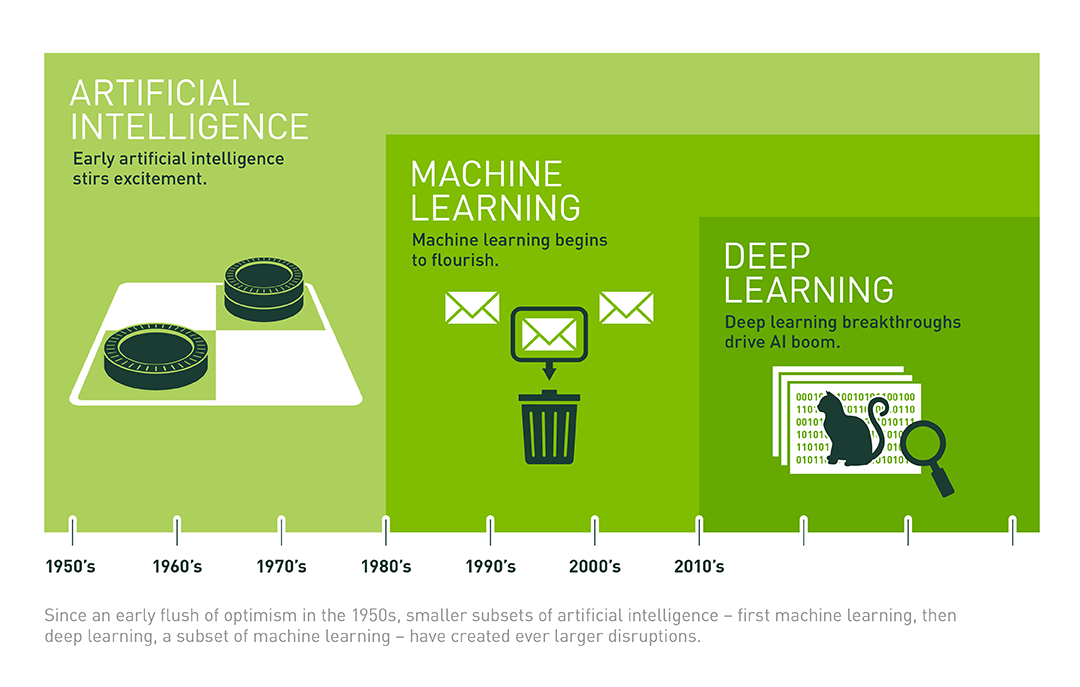
\includegraphics[width = \linewidth]{ml_dl.png}
    \caption{Mối quan hệ giữa AI, Machine Learning và Deep Learning. (Nguồn: \href{https://blogs.nvidia.com/blog/2016/07/29/whats-difference-artificial-intelligence-machine-learning-deep-learning-ai/}{What’s the Difference Between Artificial Intelligence, Machine Learning, and Deep Learning?})}
    \label{fig1}
\end{figure}
\subsection*{Hàm mất mát - Loss function}
Một mô hình Machine Learning hoàn chỉnh buộc phải có 4 bước như đã đề cập ở trên. Trong bước 3, để tìm ra các tham số mô hình, giống như ước lượng điểm (MLE) trong các mô hình thống kê, ta cũng phải giải thông qua một bài toán tối ưu - cực tiểu hàm mất mát. Hàm mất mát để định nghĩa một cách tổng quát nhất giống như một phép đo độ chính xác của thuật toán. Khi giá trị hàm mất mát nhỏ thì thường sẽ cho kết quả tốt, dẫn đến tính tất yếu của việc phải tối thiểu hàm mất mát.\\\\
Ví dụ: \\Trong các bài toán hồi quy, hàm mất mát của chúng thường là hàm sai số bình phương trung bình: Đo khoảng cách giữa đầu ra thực và đầu ra dự đoán $\mathcal{L}(\theta) = ||y-\hat{y}||_{p}^{2}$ \label{n2}
\phantom{a}\\\\
Một cách tổng quát, bài toán đi tìm tham số tương đương:
\begin{equation}
    \theta^* = \text{argmin}_{\theta}\mathcal{L}(\theta)
\end{equation}

\section{Gradient Descent}
Gradient Descent là một thuật toán tối ưu dùng để xác định tham số mô hình thông qua việc cực tiêu hàm mất mát. Đối chiếu với 4 phần, Gradient Descent có thể phân loại vào phần 3.\\\\
Theo lí thuyết, để tối ưu một hàm nhiều biến số, ta sẽ giải hệ các phương trình đạo hàm riêng, xác định các điểm dừng, từ đó tìm ra các điểm cực tiểu, cực đại của hàm số. Với giải tích ma trận, thì đôi khi ta có thể viết gọn hệ các phương trình trên thành những biểu thức vô cùng thẩm mĩ, gọn gàng và dễ dàng giải hơn nhiều. \\\\\textbf{Tuy nhiên}, vẫn không thể tránh được một thực tế có những hệ ta không thể giải được cụ thể! Hơn nữa, máy tính không biết giải hệ phương trình và phương trình phức tạp, cứ cho như giải được thì cũng không có lời giải chung cho mọi bài toán. Do đó, cần phải nghĩ ra một thuật toán đủ đơn giản, vừa tận dụng được những tài nguyên sẵn có của máy tính, vừa giải được bài toán được yêu cầu. Gradient Descent là một thuật toán đáp ứng được yêu cầu đó, đầu tiên chọn một \textit{điểm xuất phát} rồi tiến dần đến \textit{đích} sau mỗi vòng lặp.

\subsection{Tính "ngược" của Gradient}
Gradient, ta đã từng định nghĩa ở trong các bài trước khi sử dụng nó để xác định cạnh của các bức ảnh. 
\\\\
Một trong những đặc điểm quan trọng, đáng chú ý của Gradient là nó hướng theo chiều tăng của \textit{curve level}. Để cho dễ hiểu ta cùng xét ví dụ dưới đây.
\\\\
Ví dụ: Ta xét hàm $F(x,y) = x^2+y^2$. Đồ thị đường đồng mức của hàm số được cho như hình \ref{fig2}.
\begin{figure}[ht!]
    \centering
    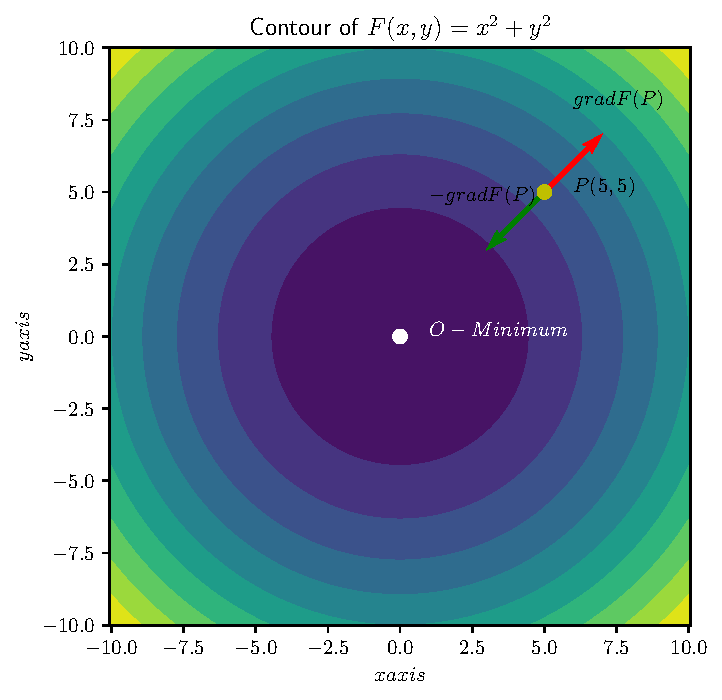
\includegraphics[width = 0.7\linewidth]{gd1.pdf}
    \caption{Tính "Ngược" của Gradient}
    \label{fig2}
\end{figure}
\phantom{a}\\\\
Dễ thấy cực tiểu của hàm số là điểm $O(0,0)$. Ta xét một điểm bất kì, ví dụ $P(5,5)$. Mũi tên màu đỏ chỉ $\nabla F(P)$, còn mũi tên màu xanh chỉ $-\nabla F(P)$. Ta có nhận xét sau:
\begin{enumerate}
    \item $\nabla F$ hướng theo chiều tăng của $z$ (chiều tăng của \textit{curve level})
    \item $\overrightarrow{PO}$ tỉ lệ với $-\nabla F(P)$ (*)
\end{enumerate}
Từ (*) ta suy ra: 
\begin{equation}
    \textbf{x}_O = \textbf{x}_P - \eta{\nabla F(P)}
    \label{eq2}
\end{equation}
Trong công thức (\ref{eq2}), $\eta$ là số mà ta không biết ta hoàn toàn có thể lựa chọn trước, nếu lần cập nhật này không tới được \textit{đích} thì ta tiếp tục lặp lại quá trình đó cho tới khi đến \textit{đích} đủ gần thì dừng. \\\\
Ta suy ra công thức cập nhật cho thuật toán Gradietn Descent:
\begin{equation}
    \theta \leftarrow  \theta - \eta{\nabla_{\theta}}f(\theta)
    \label{eq3}
\end{equation}
\underline{Lưu ý}: $\eta$ được gọi là tốc độ học (\textit{learning rate}), tốc độ học phải được điều chỉnh một cách phù hợp đảm bảo sao cho đến được \textit{đích}. Nếu $\eta$ quá nhỏ, thì phải mất rất nhiều vòng lặp mới đến được \textit{đích}. Nếu $\eta$ quá lớn, thì có thể \ldots sẽ không bao giờ đến được \textit{đích}. (Hình \ref{fig3})
\begin{figure}[ht!]
  \centering
  \begin{subfigure}[b]{\linewidth}
    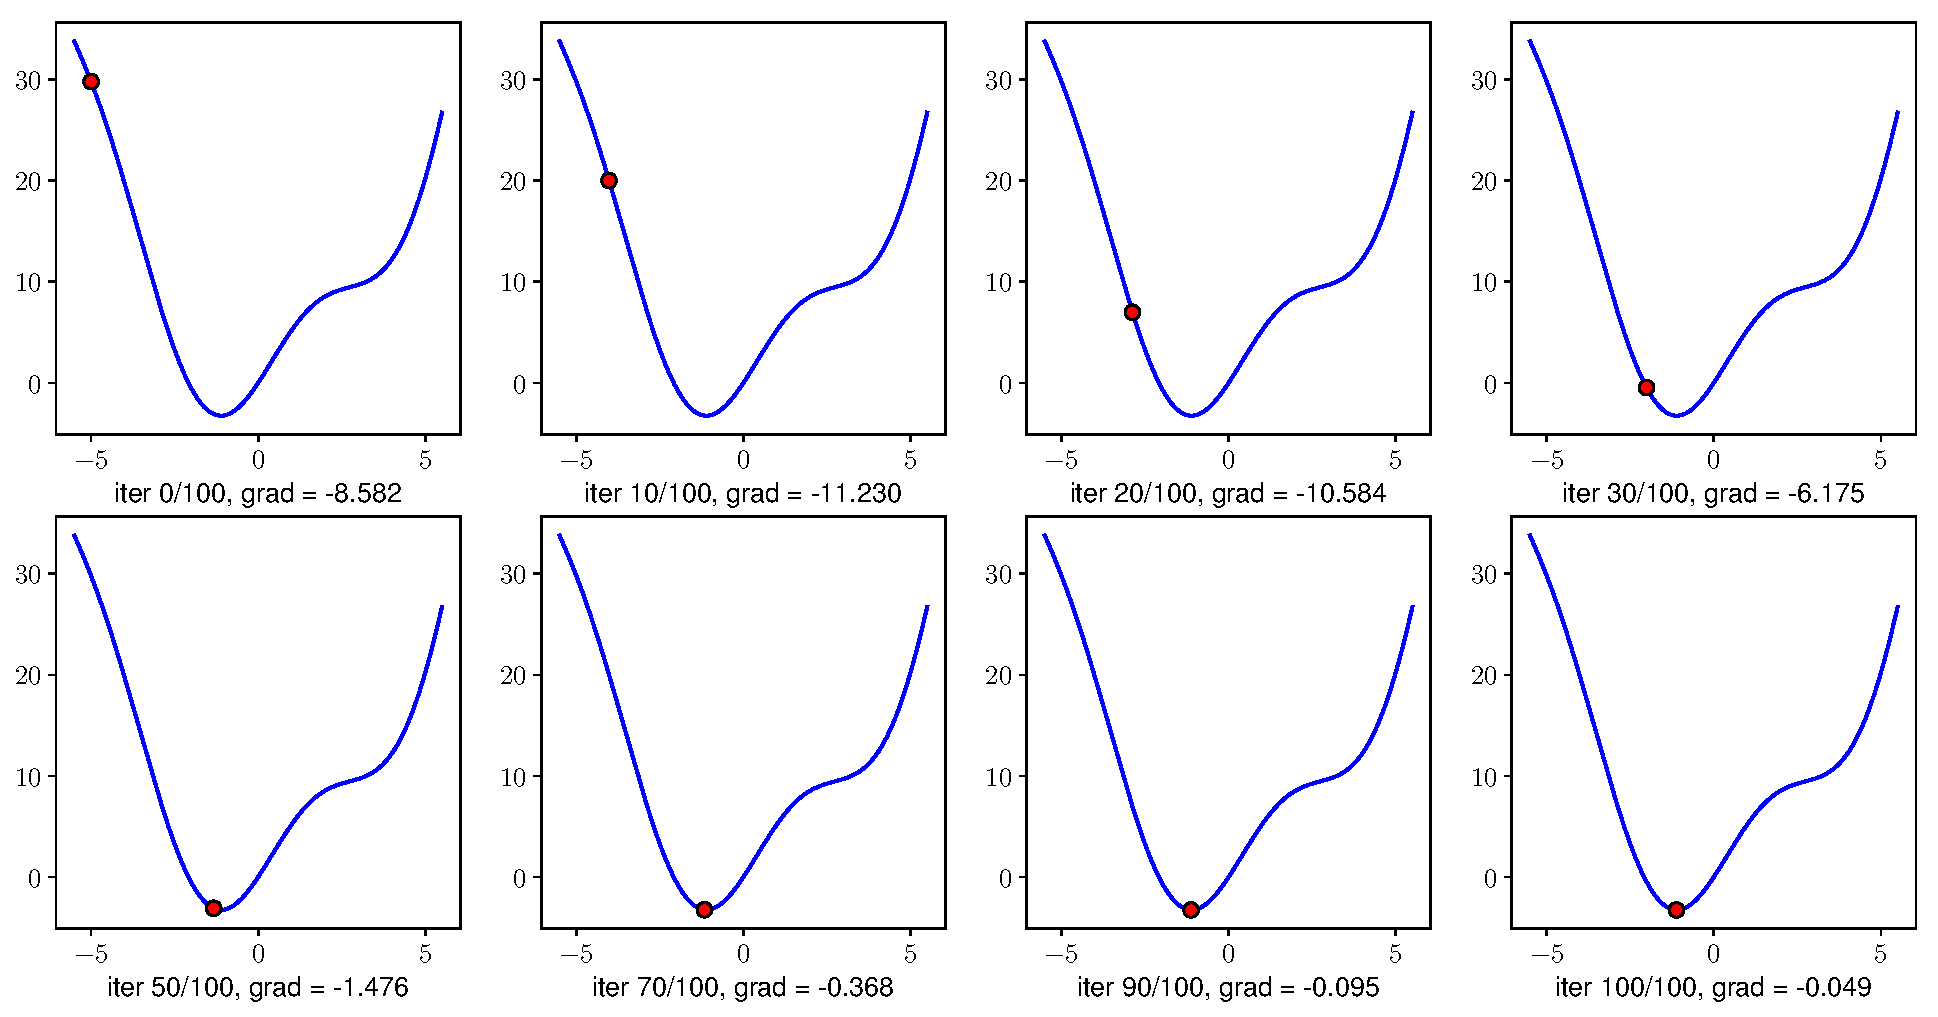
\includegraphics[width=\linewidth]{gd1d_1.pdf}
    \caption{Kết quả tìm được qua các vòng lặp với $x_0 = -5$, $\eta = 0.01$}
  \end{subfigure}
  \begin{subfigure}[b]{\linewidth}
    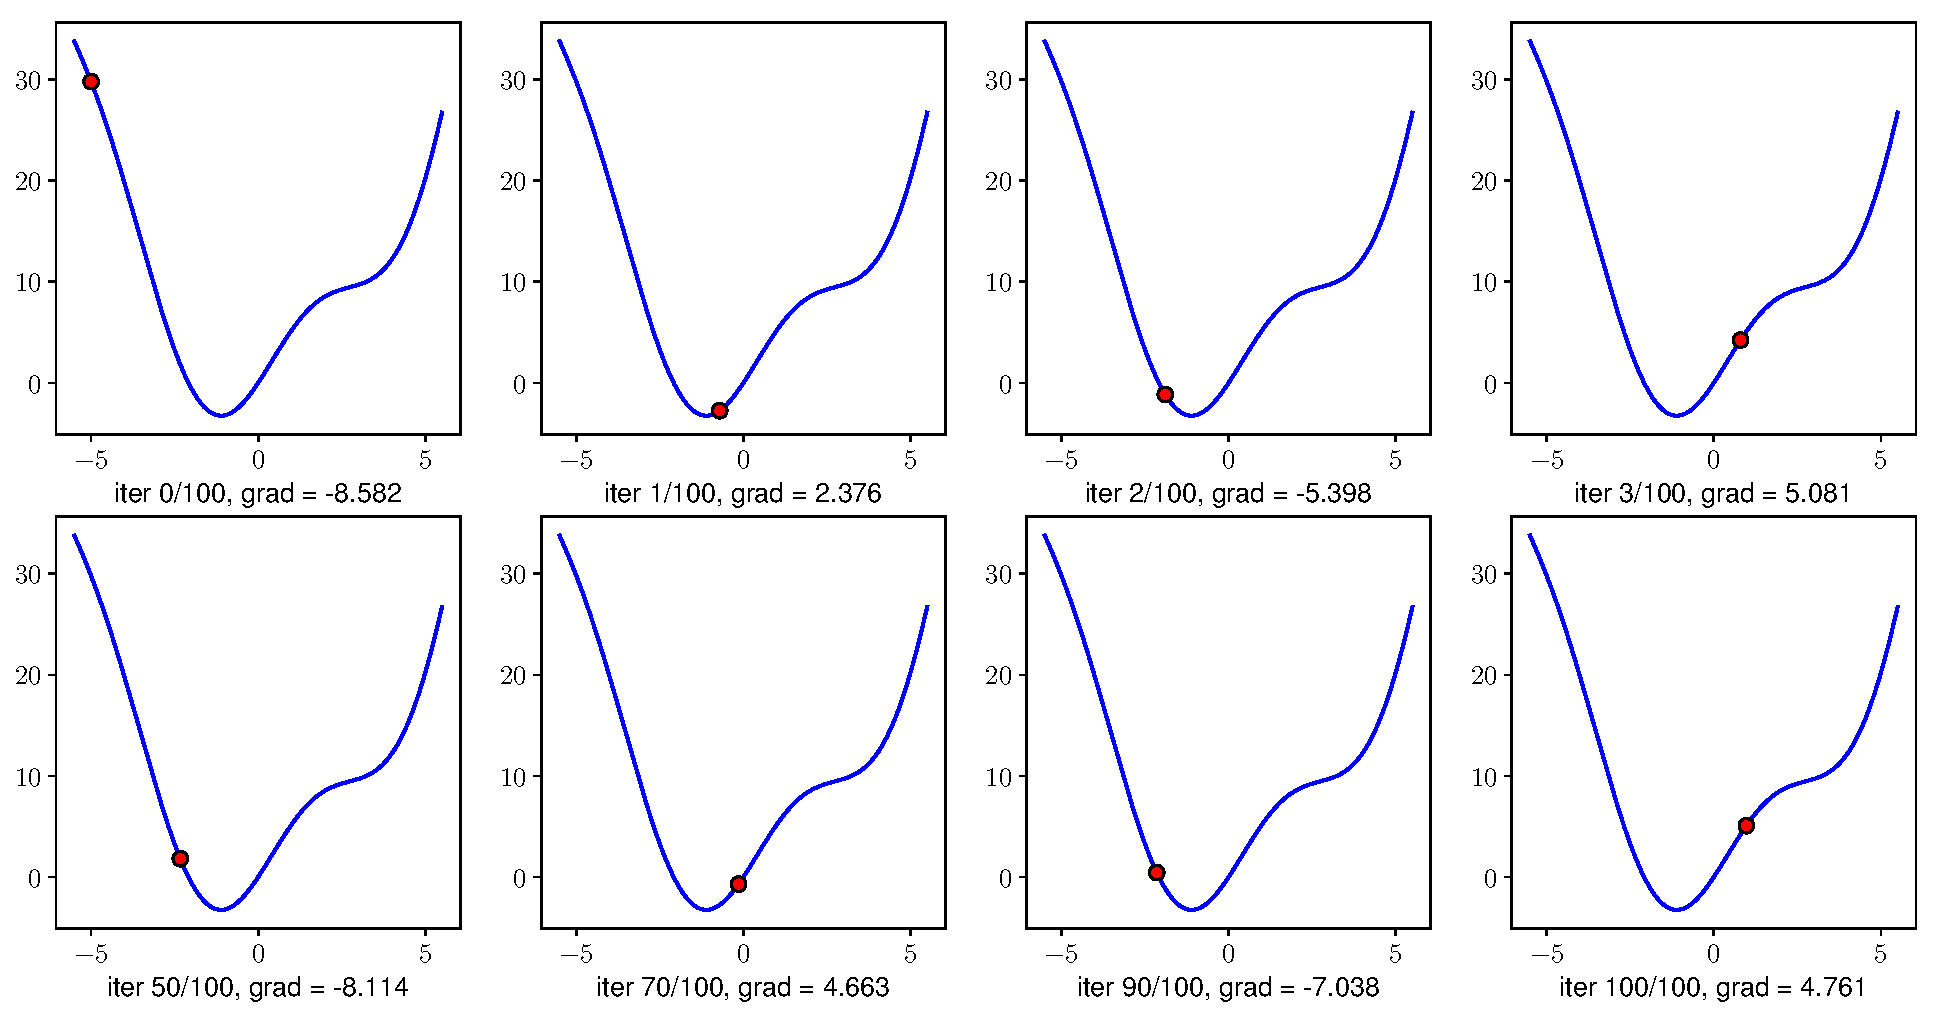
\includegraphics[width=\linewidth]{gd1d_2.pdf}
    \caption{Kết quả tìm được qua các vòng lặp với $x_0 = -5$, $\eta = 0.5$}
  \end{subfigure}
  \caption{Nguồn: machinelearningcoban.com}
  \label{fig3}
\end{figure}
\subsection{Một số biến thể của Gradient Descent}
Trong thực tế, để tăng tốc độ hội tụ cho các thuật toán Gradient Descent, có nhiều biến thể của nó được ra đời có thể kể đến: \textit{Gradient Descent with momentum}, \textit{Nesterov accelerated gradient}, \ldots
\\\\
Điều thú vị là những biến thể này cho ta một cái nhìn rất "lạ", đó là nhìn toán dưới con mắt của vật lí, biến những lí thuyết tưởng chừng như trừu tượng, xa xôi mà trở nên gần gũi đến lạ thường!\\\\
Do giới hạn về thời gian, phần này tôi xin phép được bỏ ngỏ, hẹn sẽ hoàn thiện trong tương lai gần. Code cho phần này tôi đã làm đăng lên trên github. Bạn đọc có thể tham khảo thêm ở các tài liệu tham khảo cuối bài viết.
\subsection{Stochastic gradient descent}
\subsubsection{Batch gradient descent}
Thuật toán GD được đề cập bên trên được gọi là \textit{batch gradient descent}, ta sử dụng tất cả điểm dữ liệu $\textbf{x}_i$ để cập nhật cho bộ tham số. Nhược điểm của nó là nó sẽ lâu, và mất thời gian do phải lặp đi lặp lại liên tục trên một cơ sở dữ liệu lớn. Điều này không phù hợp với những mô hình có cơ sở dữ liệu được cập nhật liên tục, việc này yêu cầu mô hình cũng cần phải cập nhật lại để phù hợp với dữ liệu mới.\\\\
Một kĩ thuật đơn giản hơn là \textit{stochastic gradient descent} (SGD) phù hợp hơn trong trường hợp này.
\subsubsection{Stochastic gradient descent}
Thuật toán này sẽ sử dụng một điểm dữ liệu $\textbf{x}_i$ cho mỗi lần cập nhật. Tuy đơn giản nhưng lại tỏ ra vô cùng hiệu quả.
\subsubsection*{epoch}
Mỗi lần duyệt qua một lượt tất cả các điểm trên toàn bộ dữ liệu được gọi là một \textit{epoch}. Với GD thông thường, mỗi epoch ứng với một lần cập nhật $\theta$, còn đối với SGD thì ứng với $N$ lần cập nhật $\theta$. Tuy nhiên SGD có thể hội tụ nhanh hơn nhiều, chỉ một vài epoch. Điều này phù hợp với các bài toán yêu cầu mô hình thay đổi liên tục, với các bộ tham số đã được huấn luyện, khi thêm dữ liệu, ta có thể chạy thêm một vài epoch nữa là đã có nghiệm hội tụ
\begin{equation}
    \theta \leftarrow \theta - \eta \nabla_{\theta} J{(\theta;\textbf{x}_i, \textbf{y}_i)}
    \label{eq4}
\end{equation}
Công thức (\ref{eq4}) là công thức cập nhật cho thuật toán SGD. \\\\
\underline{Lưu ý}: Thứ tự lấy các điểm dữ liệu cần được xáo trộn để đảm bảo tính ngẫu nhiên. Việc này cũng ảnh hưởng tới hiệu năng của SGD. Đây cũng là bắt nguồn của từ \textit{stochastic}. Ngoài ra, các thuật toán tăng tốc GD như momentum hay NAG cũng có thể áp dụng cho SGD.
\subsubsection{Mini-batch gradient descent}
Từ cái tên ta hiểu, trong thuật toán này ta sẽ làm việc với các lô nhỏ hơn. Tức ta sẽ chia tập dữ liệu ban đầu thành nhiều lô nhỏ, sau đó cập nhật theo từng lô nhỏ! Còn lại thuật toán này hầu như giống SGD!

\subsection{Điều kiện dừng thuật toán}
Trong thực nghiệm, ta có thể kết hợp sử dụng các phương pháp sau:
\begin{enumerate}
    \item Giới hạn số vòng lặp.
    \item So sánh gradient của hàm mất mát tại hai lần cập nhật liên tiếp tiếp, đủ nhỏ thì dừng lại.
    \item So sánh gradient sau một vài epoch, đủ nhỏ thì dừng lại
    \item Kết hợp kiểm tra trên tập xác thực và tập huấn luyện, nếu chất lượng mô hình bắt đầu giảm trên tập xác thực thì dừng lại.
\end{enumerate}

\section{Some simple neural network models}
\subsection{Neural network?}
\begin{figure}[ht!]
    \centering
    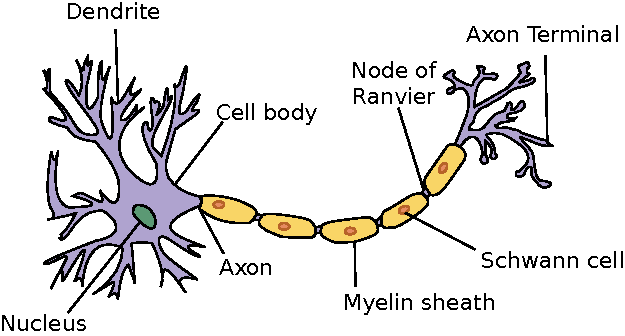
\includegraphics[width = 0.7\linewidth]{neuron.pdf}
    \caption{Mô hình mạng neuron sinh học, Nguồn: Dive into Deep Learning}
    \label{fig4}
\end{figure}
\phantom{a}\\
Hình \ref{fig4} là một mô hình mạng neuron trong thực tế. Khi nhắc tôi mô hình mạng neuron - cái tên cho ta nghĩ rằng mô hình này đã dựa trên mạng neuron sinh học, nhưng thực tế có vẻ như hơi\ldots ngược. Bởi hồi quy tuyến tình (được phát minh vào năm 1795) được phát triển trước ngành khoa học thần kinh tính toán.\\\\
Các mô hình tuyến tính chính là khởi nguồn cho các mạng neuron nhân tạo. Hãy cùng xem hình \ref{fig4}, mô hình này bao gồm \textit{sợi nhánh - Dendrite} (cổng đầu vào), \textit{nhân tế bào - Nucleus} (bộ xử lý trung tâm), \textit{sợi trục - Axon} (dây đầu ra), và \textit{đầu cuối sợi trục - Axon Terminal} (cổng đầu ra), cho phép kết nối với các tế bào thần kinh khác thông qua \textit{synapses}\footnote{Synap hóa học là nơi tiếp xúc giữa hai nơron, mà thông qua đó cho phép các nơron truyền đi thông tin qua lại lẫn nhau (chỉ một chiều)}.\\\\
Nguyên lí cơ bản như sau: thông tin ($\textbf{x}_i$) sẽ được tiếp nhận tại các sợi nhánh, sau đó sẽ được xác định các ảnh hưởng bởi \textit{synapses} (nhân với các trọng số $\textbf{w}_i$). Các thông tin  sau đó được tổng hợp lại tại nhân tế bào ($y = \sum_{i}\textbf{x}_{i}^{\text{T}}\textbf{w}_i + b$) và tiếp theo là được hậu xử lí trong các sợi trục (xử lí phi tuyến $f(y)$), cuối cùng là được gửi đến đích (ví dụ, cơ bắp) hoặc được đưa vào một tế bào thần kinh khác thông qua các sợi nhánh.\\\\ \label{n1}
Dựa trên các nghiên cứu thực tế về các hệ thống thần kinh sinh học, ta chắc chắn một điểu rằng nhiều đơn vị như vậy khi được kết hợp với nhau theo đúng cách, cùng với thuật toán học phù hợp, sẽ tạo ra các hình vi thú vị và phức tạp hơn nhiều so với bất kì neuron đơn lẻ nào có thể làm được.\\\\
Người ta cũng chứng minh được rằng mạng neuron có khả năng sấp xỉ hầu hết các hàm liên tục. Điều này thể hiện rõ tính ưu việt của một mô hình mạng neuron trong việc xây dựng một mô hình học máy nói chung và học sâu nói riêng.\\\\
\underline{Lưu ý}: Trong phạm vi bài này, chúng ta chỉ nghiên cứu các mô hình mạng neuron đơn giản, tức là các mạng neuron tuyến tính đã ra đời từ cả trăm năm về trước. Các mô hình mạng neuron hiện đại ta sẽ đề cập trong các bài sau.

\subsection{Các mạng neuron đơn giản nhất}
Từ nguyên lí cơ bản bên trên (phần \ref{n1}), ta có thể suy ra mô hình toán học của một mạng neuron tuyến tính đơn giản:
\begin{equation}
    \hat{y} = f(\sum_{i}\textbf{x}_{i}^{\text{T}}\textbf{w}_i + b)
\end{equation}
Trong đó, $\hat{y}$ là đầu ra dự đoán, $f(s)$ là hàm kích hoạt \footnote{$f(s)$ là hàm kích hoạt phi tuyến, bởi nếu $f(s)$ tuyến tính, sự xuất hiện của $f(s)$ là vô nghĩa vì ta luôn có thể biểu diễn đầu ra qua bộ tham số khác}. \\\\Trong thực tế, một mô hình mạng neuron có thể rất phức tạp với nhiều tầng ẩn/tầng trung gian giữa tầng đầu vào và tầng đầu ra. Một mô hình mạng neuron đơn giản nhất chỉ gồm tầng đầu vào, một nút đầu ra.
\begin{figure}[ht!]
    \centering
    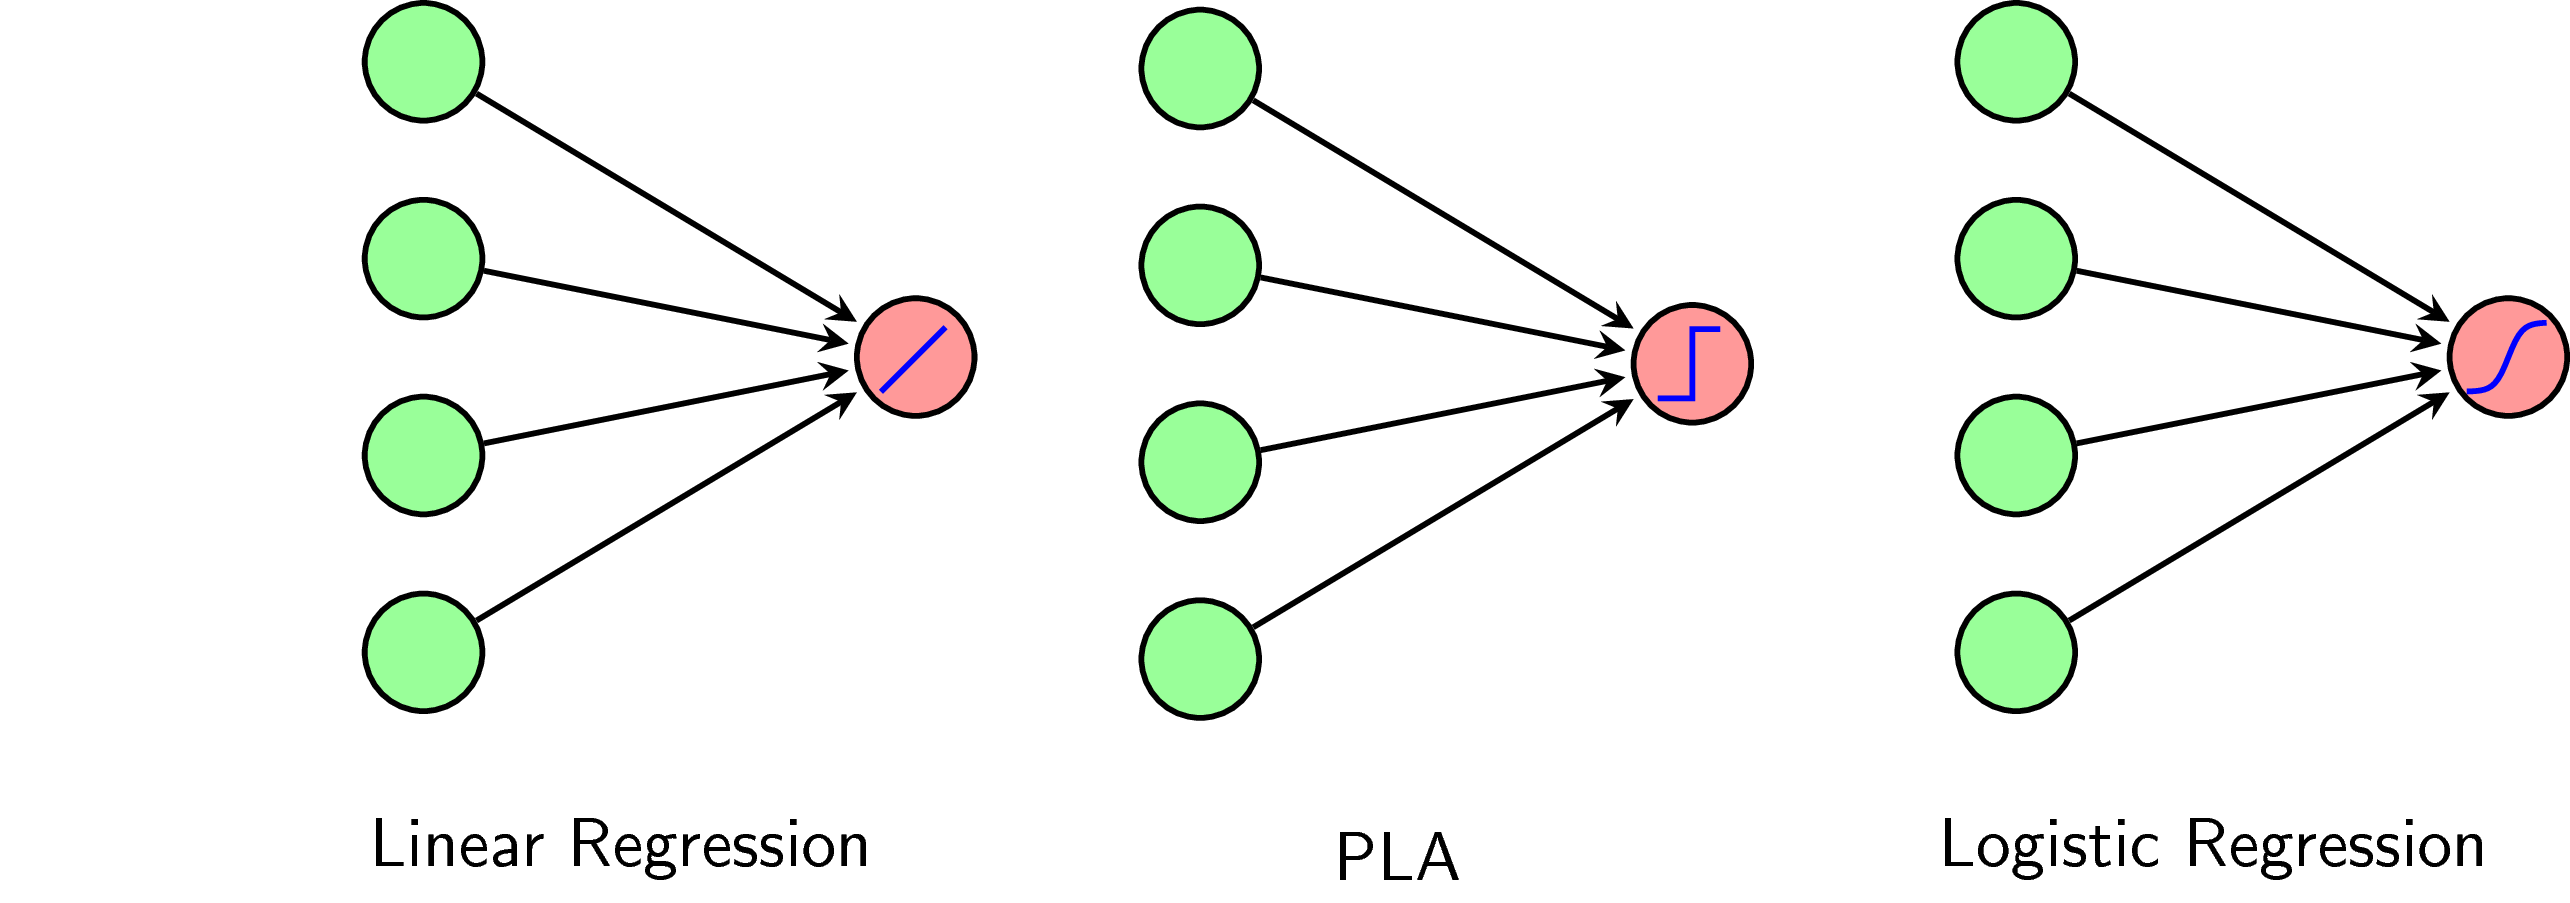
\includegraphics[width = \linewidth]{3models.png}
    \caption{Các mô hình mạng neuron đơn giản nhất, Nguồn: machinelearningcoban.com}
    \label{fig5}
\end{figure}
\phantom{a}\\
Hình \ref{fig5} minh họa cho cấu trúc của các mô hình mạng neuron đơn giản. Về bản chất, chúng như nhau, chỉ khác nhau ở hàm kích hoạt $f(s)$.\\\\
Sau đây ta sẽ đi vào thực hành và quan sát ba mô hình trên, các bản chất toán học bên trong nó, qua đó hiểu một cách đơn giản về cách hoạt động của một mô hình mạng neuron, nền tảng cho những mô hình phức tạp hơn sau này!

\subsubsection{Linear Regression}
Lược qua về lịch sử, Hồi quy tuyến tính có lẽ là công cụ đơn giản nhất và phổ biến nhất để giải quyết các vấn đề về hồi quy. Ra đời từ những năm đầu của thế kỉ 19 (Gauss, 1809, Lengendre, 1805).\\\\
Ta đã từng đề cập qua phép nội suy tuyến tính trong các phép biến đổi hình học. Ở đây hồi quy tuyến tính cũng khá tương tự, ý tưởng là ta sẽ giả sử rằng mối quan hệ giữa các đặc trưng ($\textbf{x}$) và nhãn ($y$) của chúng có mối qua hệ xấp xỉ tuyến tính. Theo ngôn ngữ của xác suất thống kê, thì hồi quy tuyến tính được viết dưới dạng $Y = X\textbf{w}+b$. Nếu ta coi như ta có thể kiểm soát hoàn toàn được $X$, thì biểu thức trên được viết lại dưới dạng kì vọng có điều kiện của $Y$, $E(Y|X=\textbf{x}) = \textbf{x}^{\text{T}}\textbf{w}+b$, tức là tổng có trọng số của các đặc trưng $\textbf{x}$. Cách biểu diễn trên thỏa mãn rằng các nhãn thực tế vẫn có thể lệch so với đường thẳng kì vọng bởi nhiễu $Y = \textbf{x}^{\text{T}}\textbf{w}+b+\varepsilon$ (*).
\\\\
Trong thực tế, việc giả sử như $\textbf{x}$ đã được xác định có phần không thật hợp lí. Tuy nhiên có thể yêu cầu tính bất định của $X$ là không đáng kể so với $Y$ (mà thực nghiệm có thể chấp nhận được), hơn nữa vế phải của (*) đã có tính ngẫu nhiên, những khía cạnh ngẫu nhiên của $X$ có thể trong một chừng mực nào đó chuyển sang cho nhiễu. Và ta có thể giả sử các nhiễu tuân theo phân phối chuẩn (Gaussian distribution).
\subsubsection*{Hàm mất mát - Loss Function}
Hàm mất mát phổ biến cho các bài toán hồi quy thường là hàm sai số bình phương trình bình (MSE) như đã giới thiệu trong ví dụ ở phần \ref{n2}.
\begin{equation}
    J(\textbf{w}) = \frac{1}{2N}\sum_{i}^{N}{||\hat{y_i}-y_i||}_{2}^{2}=\frac{1}{2N}\sum_{i}^{N}{||\textbf{x}_{i}^{\text{T}}\textbf{w}-y_i||_{2}^{2}}
    \label{eq6}
\end{equation}
Trong công thức (\ref{eq6}) ta cần lưu ý:
\begin{enumerate}
    \item chia cho $2N$ vừa để đảm bảo cho khái niệm "trung bình" vừa để tránh dư thừa hệ số 2 sau khi đạo hàm.
    \item \textbf{w} ở đây đã gộp cả hệ số $b$ (bias trick). Khi đó \textbf{x} sẽ có dạng $[x_1;x_2;\ldots;x_d,1]$
\end{enumerate}
\begin{figure}[ht!]
    \centering
    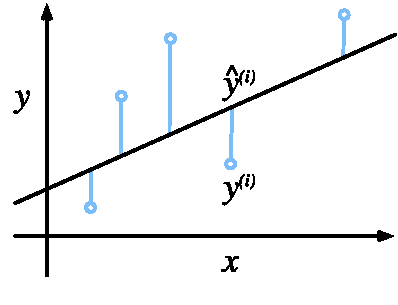
\includegraphics[width = 0.5\linewidth]{fit-linreg.pdf}
    \caption{Đường thẳng tốt nhất cho hồi quy tuyến tính một chiều, Nguồn: Dive into Deep Learning}
    \label{fig6}
\end{figure}
\phantom{a}\\
Sau đó nhiệm vụ của chúng ta, đó là đi tìm bộ tham số mô hình \textbf{w}. Tức là ta phải giải bài toán tối ưu sau:
\begin{equation}
    \textbf{w}^* = \text{argmin}_{\textbf{w}}J(\textbf{w})
\end{equation}
Khi đó, mô hình hồi quy tuyến tính (đường thẳng tốt nhất) của chúng ta chính là $y = \textbf{x}^{\text{T}}\textbf{w}^{*}$\\\\
Hình \ref{fig6} cho ta ví dụ về mô hình hồi quy tuyến tính một chiều.
\subsubsection*{Analytic Solution}
Hồi quy tuyến tính\ldots vô tình lại là một mô hình có thể tối ưu trực tiếp hàm mất mát bằng các công cụ toán học như giải tích ma trận!
\\\\
Từ công thức (\ref{eq6}), ta có thể biến đổi tiếp hàm mất mát tương đương
\begin{equation}
    J(\textbf{w}) = \frac{1}{2N}||\textbf{X}\textbf{w}-\textbf{y}||_{2}^{2}
    \label{eq8}
\end{equation}
Lưu ý rằng, \textbf{X} là ma trận tạo bởi sự xếp chồng giữa các điểm dữ liệu, có kích thước $N\times(d+1)$, $d+1$ do \textit{bias trick}.\\\\
Ta có,
\begin{equation}
    \nabla J(\textbf{w}) = \frac{1}{N} \textbf{X}^{\text{T}}(\textbf{X}\textbf{w}-\textbf{y})
    \label{eq9}
\end{equation}
Phương trình gradient bằng không:
\begin{equation}
    \nabla J(\textbf{w}) = 0 \Leftrightarrow \textbf{X}^{\text{T}}\textbf{X}\textbf{w}=\textbf{X}^{\text{T}}\textbf{y}
    \label{eq10}
\end{equation}
Phương trình (\ref{eq10}) để giải được trong mọi trường hợp ta cần thêm khái niệm \textit{giả nghịch đảo - Pseudo-Inverse}, chính là tổng quát hơn của khái niệm nghịch đảo. Khi đó ta có thể giải ra được \textbf{w} như sau:
\begin{equation}
    \textbf{w} = \left(\textbf{X}^{\text{T}}\textbf{X} \right)^{\dagger}\textbf{X}^{\text{T}}\textbf{y}
\end{equation}
\subsubsection*{Gradient descent}
Hồi quy tuyến tính có một sự đặc biệt không hề nhẹ trong việc giải phương trình tối ưu. Tuy nhiên ta sẽ không theo đuổi mục đích đó như đã nói trong phần Gradient descent. Bài toán này ta có thể giải bằng SGD hoặc Mini-batch GD.
\\\\
\textbf{SGD}\\\\
Công thức cập nhật cho SGD như sau:
\begin{equation}
    \textbf{w} \leftarrow \textbf{w} - \eta. \textbf{x}^{\text{T}}(\textbf{x}\textbf{w}-y)
    \label{eq12}
\end{equation}
\textbf{Mini-batch GD}\\\\
Công thức cập nhật cho Mini-batch GD như sau:
\begin{equation}
    \textbf{w} \leftarrow \textbf{w} - \eta. \frac{1}{N_b} \textbf{X}_{b}^{\text{T}}(\textbf{X}_{b}\textbf{w}-\textbf{y})
\end{equation}
\begin{figure}[ht!]
    \centering
    \begin{subfigure}[b]{0.45\linewidth}
        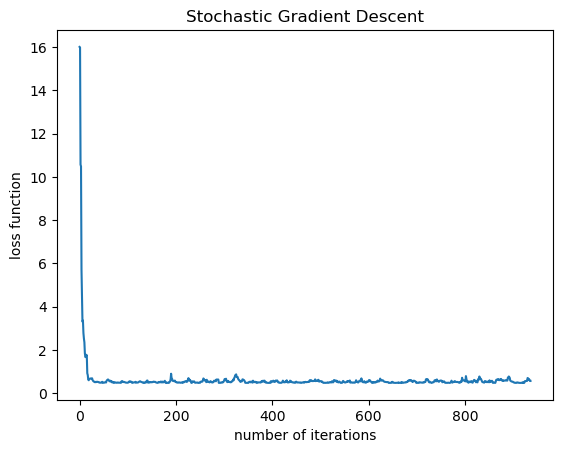
\includegraphics[width = \linewidth]{linear_sgd.png}
        \caption{Sử dụng SGD}
        \label{fig7a}
    \end{subfigure}
    \begin{subfigure}[b]{0.45\linewidth}
        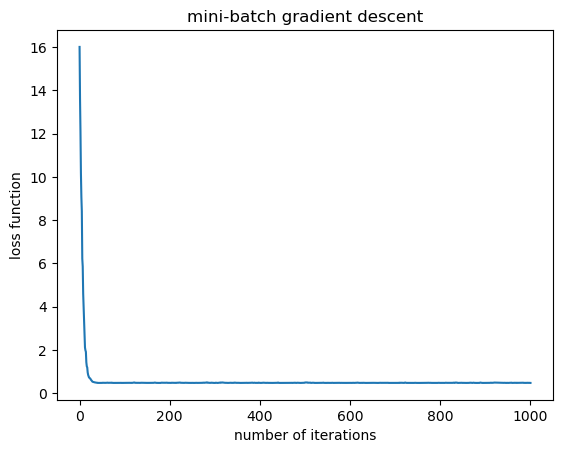
\includegraphics[width = \linewidth]{linear_mgd.png}
        \caption{Sử dụng mini-batch GD}
        \label{fig7b}
    \end{subfigure}
    \caption{Giá trị của hàm mất mát sau mỗi vòng lặp}
    \label{fig7}
\end{figure}
\subsubsection*{Mô hình mạng neuron}
Mô hình mạng neuron của hồi quy tuyến tính có thể được biễu diễn như trong hình \ref{fig12}
\begin{figure}[ht!]
    \centering
    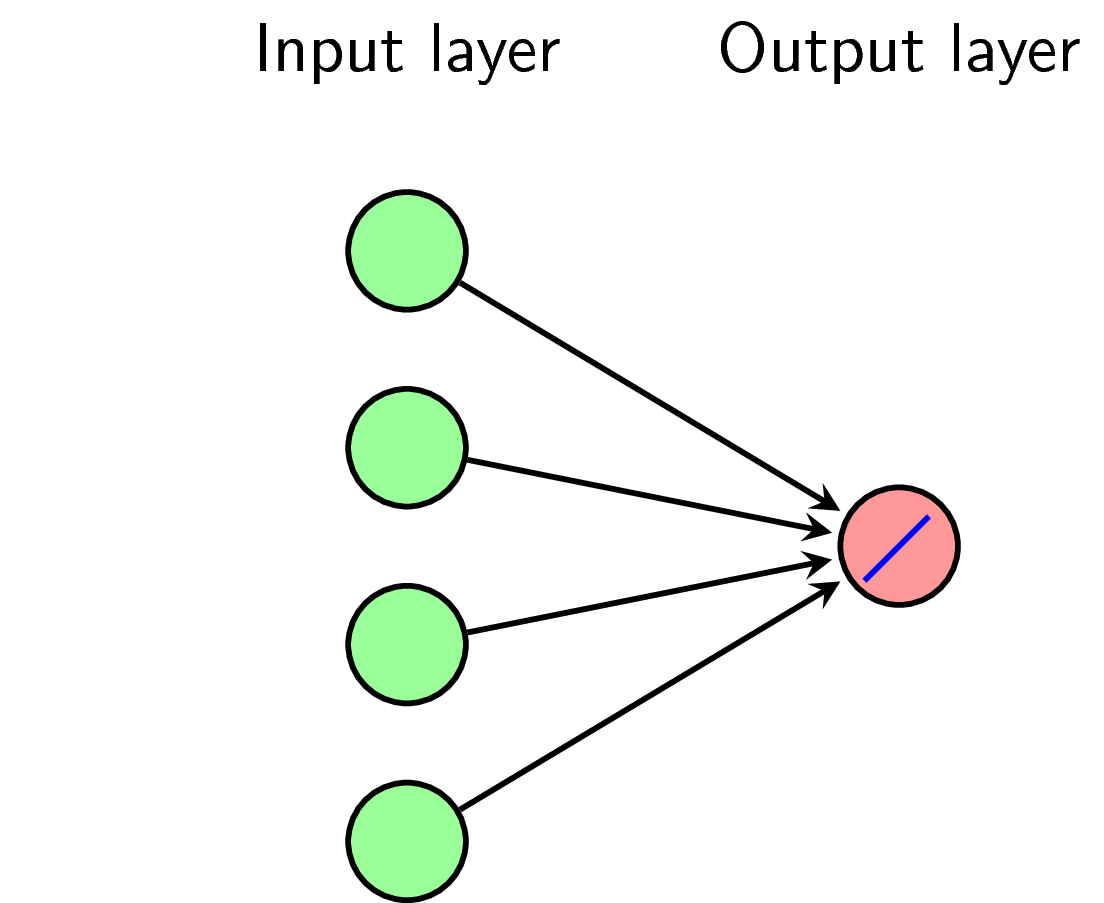
\includegraphics[width = 0.4\linewidth]{lr_nn.png}
    \caption{Biểu diễn hồi quy tuyến tính dưới dạng mạng neuron. Nguồn: machinelearningcoban.com}
    \label{fig12}
\end{figure}
\phantom{a}\\
Hàm kích hoạt khi đó là $f(s) = s$ là một hàm tuyến tính, cho nên có thể bỏ qua sự có mặt của hàm kích hoạt!

\subsubsection{Perceptron}
\textit{Thuật toán học perceptron} (perceptron learning algorithm - PLA) là một trong những thuật toán xuất hiện đầu tiên trong lịch sử machine learning. \\\\Đây là một thuật toán đơn giản giúp tìm ranh giới siêu phẳng cho bài toán phân loại nhị phân trong trường hợp tồn tại siêu phẳng đó. Nếu hai tập dữ liệu có thể được phân chia hoàn toàn bằng một siêu phẳng, ta nói rằng hai tập đó \textit{tách biệt tuyến tính} (linear separable).

\begin{figure}[ht!]
    \centering
    \begin{subfigure}[b]{0.45\linewidth}
        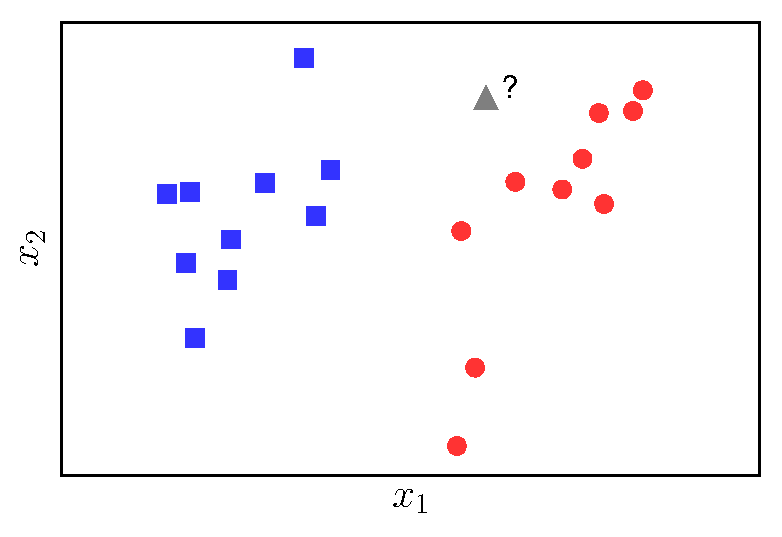
\includegraphics[width = \linewidth]{pla1.pdf}
        \label{fig8a}
    \end{subfigure}
    \begin{subfigure}[b]{0.45\linewidth}
        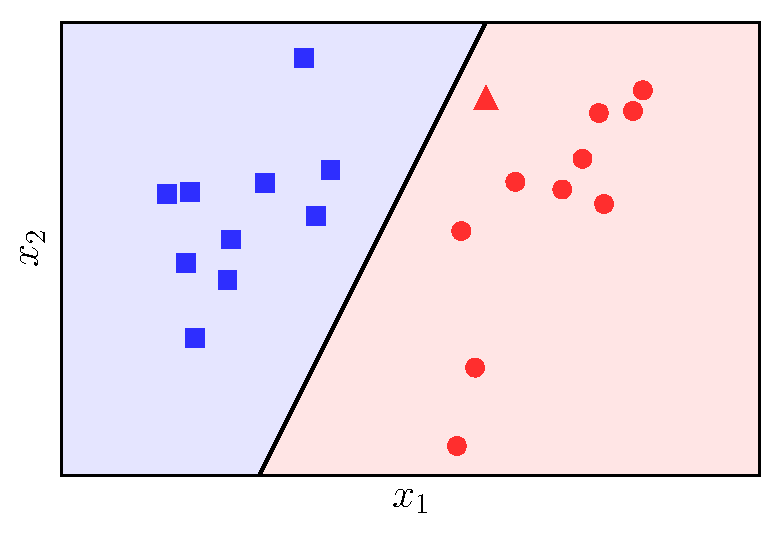
\includegraphics[width = \linewidth]{pla2.pdf}
        \label{fig8b}
    \end{subfigure}
    \caption{Bài toán phân loại nhị phân trong không gian hai chiều. (a) Cho hai tập dữ liệu được gán nhãn vuông và tròn, hãy xác định nhãn của điểm tam giác. (b) Ví dụ về một ranh giới phẳng phân chia hai tập hợp. Điểm tam giác được phân vào tập các điểm hình tròn. Nguồn: machinelearningcoban.com}
    \label{fig8}
\end{figure}
\subsubsection*{Hàm mất mát - Loss Function }
Trước tiên ta phải quy ước gán nhãn cho các điểm. Với nhận xét rằng, các điểm nằm cùng nằm về một phía của đường thẳng thì có cùng dấu. Ta có thể quy ước nhãn của chúng như sau:
\begin{equation}
    \text{label(\textbf{x})} = \begin{cases}
1, \text{ if } \textbf{x}^{\text{T}}\textbf{w} \geq 0\\
-1, \text{ o.w}
    \end{cases}
    \label{eq14}
\end{equation}
Vậy, $\text{label}(\textbf{x}) = \text{sgn}(\textbf{x}^{\text{T}}\textbf{w})$
. Từ việc gán nhãn như trên, một điểm mà bị phân loại lỗi có đặc điểm đó là tích $y_i.\textbf{x}^{\text{T}}\textbf{w}<0$ 
\\\\
Khi đó ta có thể xây dựng hàm mất mát như sau:
\begin{equation}
    J(\textbf{w}) = \sum_{\textbf{x}_i \in M} (-y_i.\textbf{x}^{\text{T}}\textbf{w})
\end{equation}
Trong đó tập $M$ là tập hợp các điểm phân loại lỗi.
\subsubsection*{Gradient descent}
Bài này SGD là lựa chọn hợp lí nhất. Với công thức cập nhật đơn giản như sau:
\begin{equation}
    \textbf{w} \leftarrow \textbf{w}+y_i\textbf{x}_i
\end{equation}
 \begin{figure}[ht!]
     \centering
     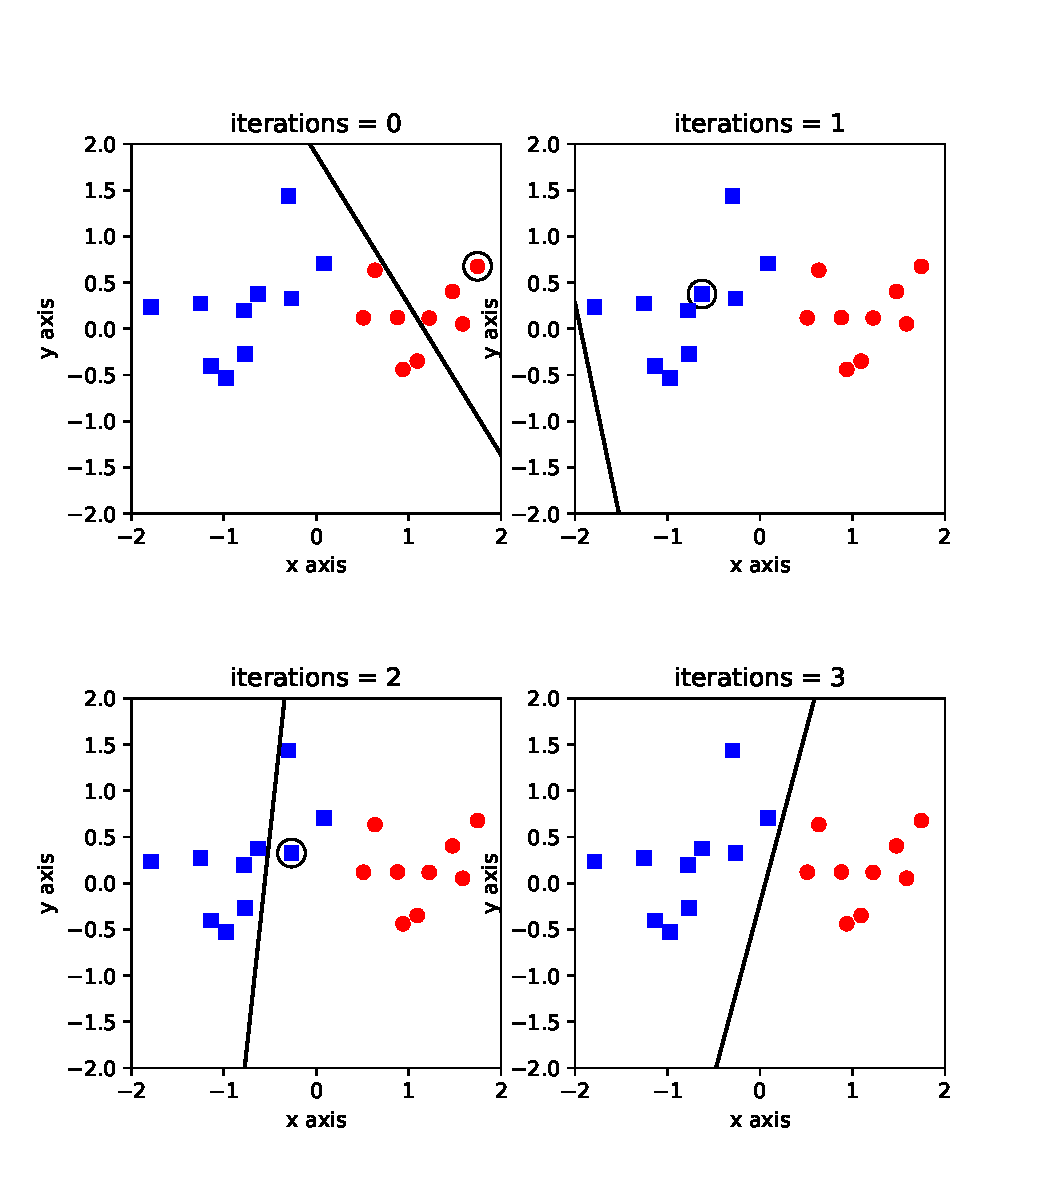
\includegraphics[width = 0.8\linewidth]{perceptron2.pdf}
     \caption{Quá trình làm việc của thuật toán, các điểm khoanh tròn là các điểm bị phân loại lỗi.}
     \label{fig9}
 \end{figure}
 \subsubsection*{Sự hội tụ}
 Thuật toán PLA chỉ hội tụ khi dữ liệu của ta \textit{tách biệt tuyến tính}. Do đó PLA có thể có vô số nghiệm (Hình \ref{fig10a}) hoặc vô nghiệm (thậm chí với nhiễu nhỏ) (Hình \ref{fig10b})
 \begin{figure}[ht!]
    \centering
    \begin{subfigure}[b]{0.45\linewidth}
        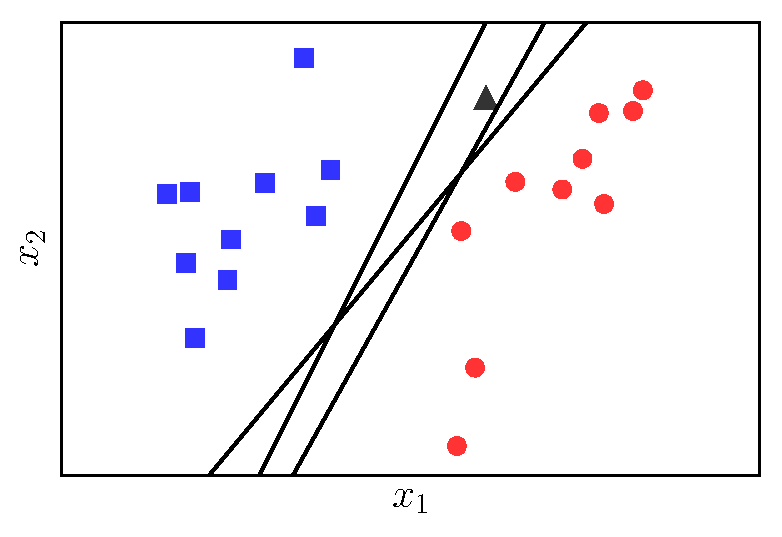
\includegraphics[width = \linewidth]{pla6.pdf}
        \caption{}
        \label{fig10a}
    \end{subfigure}
    \begin{subfigure}[b]{0.45\linewidth}
        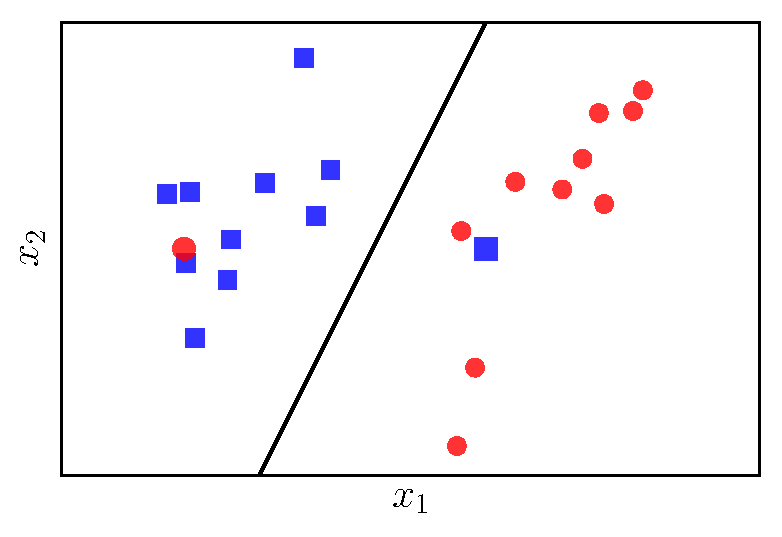
\includegraphics[width = \linewidth]{pla7.pdf}
        \caption{}
        \label{fig10b}
    \end{subfigure}
    \caption{Vấn đề hội tụ PLA, Nguồn: machinelearningcoban.com}
    \label{fig10}
\end{figure}

\subsubsection*{Mô hình mạng neuron}
\begin{figure}[ht!]
    \centering
    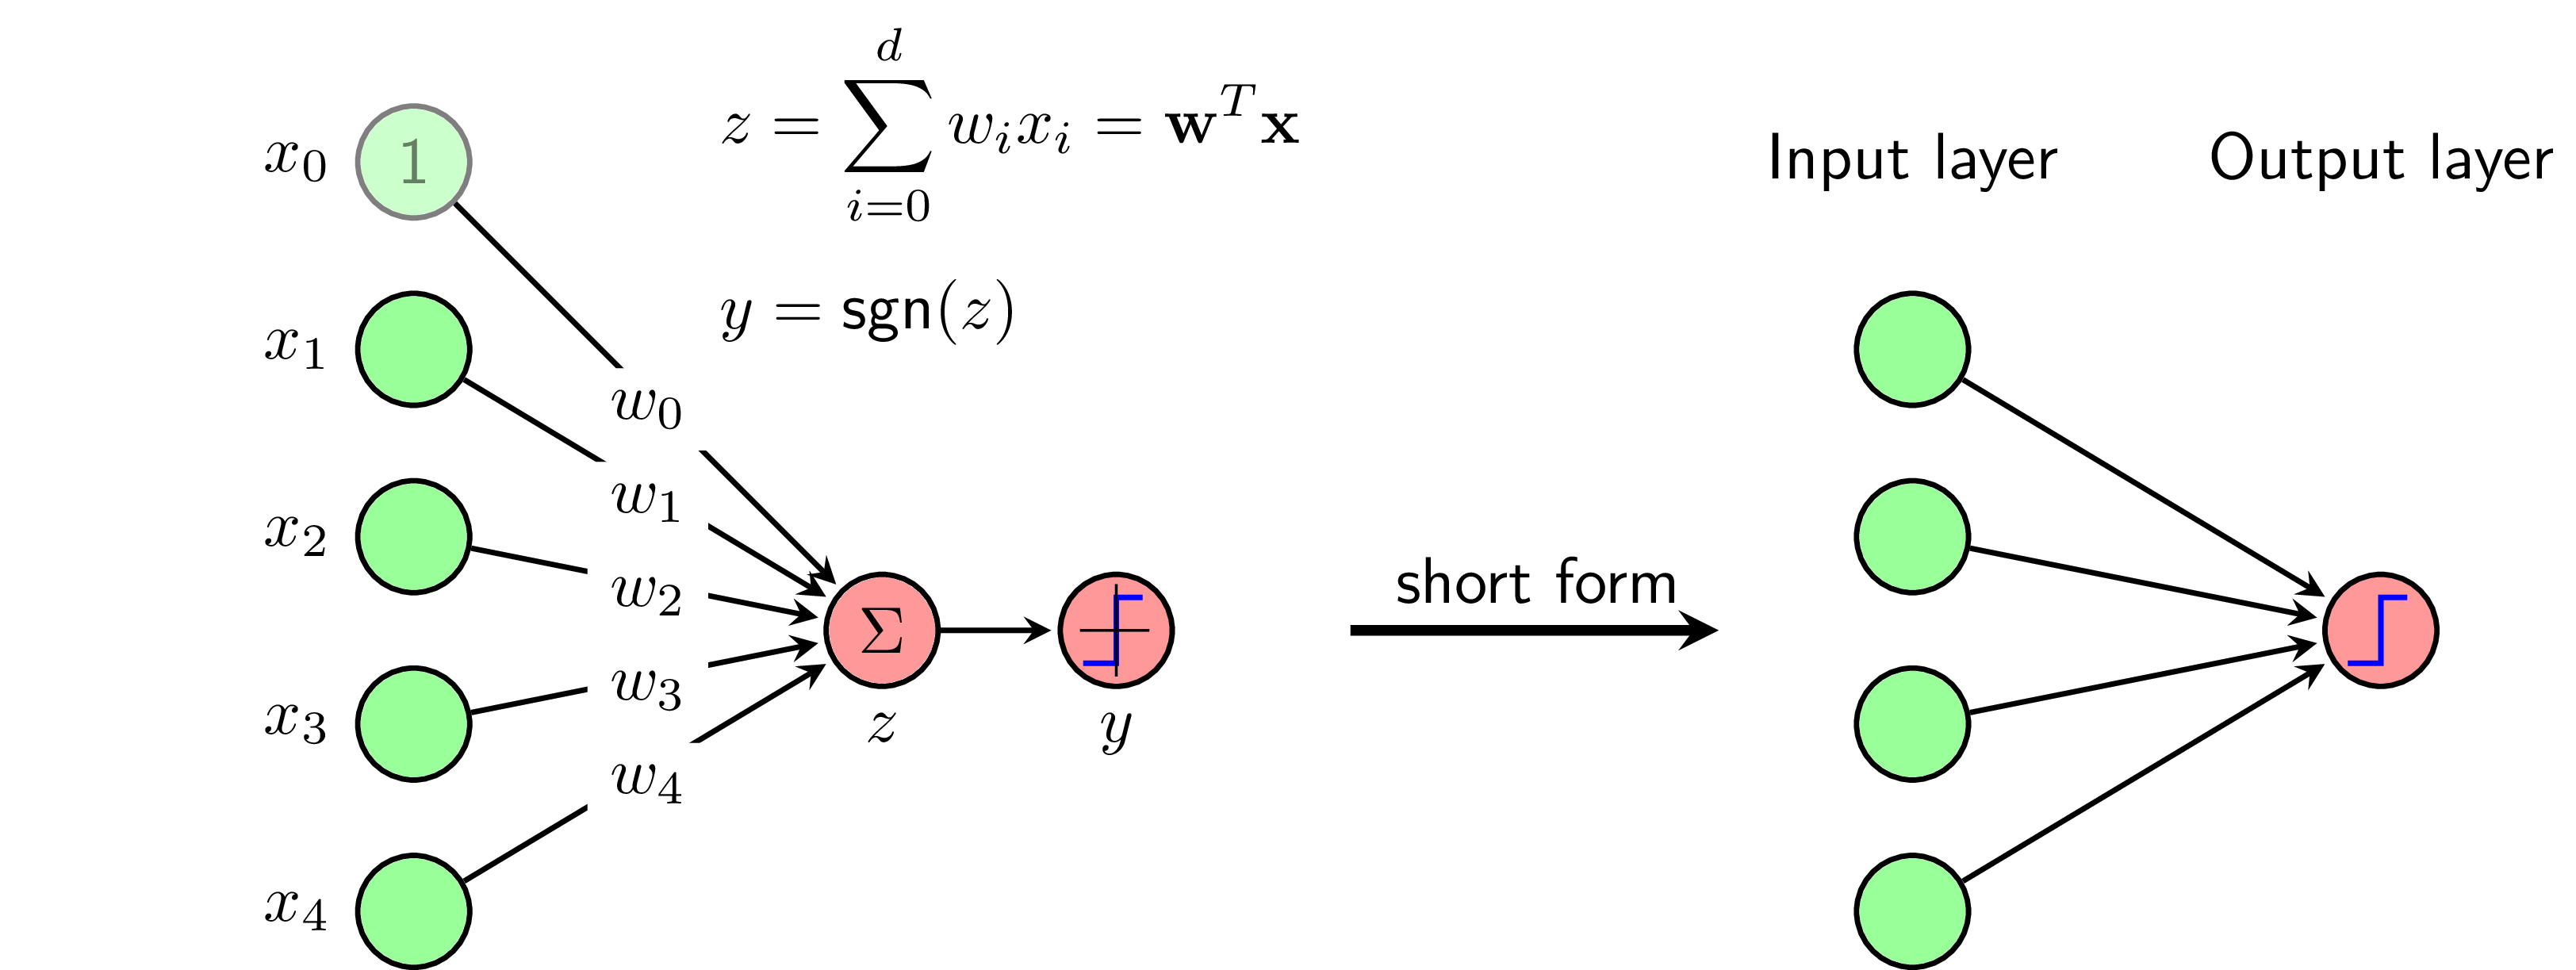
\includegraphics[width = \linewidth]{pla_nn.png}
    \caption{Biểu diễn PLA dưới dạng mạng neuron. Nguồn: Machinelearningcoban.com}
    \label{fig11}
\end{figure}
\phantom{a}\\
Hình \ref{fig11} biễu diễn mô hình mạng neuron của PLA. Cũng giống như hồi quy tuyến tính, sự khác nhau duy nhất nằm ở hàm kích hoạt $f(s) = \text{sgn}(s)$.
\subsubsection{Logistic Regression}
Trong mục này chúng ta cũng sẽ tiếp tục thảo luận về một mô hình tuyến tính khác, thường được sử dụng cho các bài toán phân loại nhị phân. Trong mô hình này đầu ra có thể được biểu diễn dưới dạng xác suất. Mô hình này có tên là \textit{hồi quy logistic}, mặc dù trong tên có chứa từ \textit{hồi quy}, song, phương pháp này thường được sử dụng trong các bài toán phân loại.\\\\
Như chúng ta đã biết thì PLA cũng được sử dụng cho mục đích phân loại nhị phân. Tuy nhiên điều kiện hội tụ của nó buộc các điểm dữ liệu phải tách biệt tuyến tính, mô hình sẽ vô nghiệm cho dù chỉ là nhiễu nhỏ.\\\\
Để giải thích do điều này, ta có thể cho rằng do ngưỡng phân loại của PLA quá cứng và ngặt! Không đủ "nhạy cảm"!\\\\
Ta cùng xét ví dụ sau: Nghiên cứu số giờ học và kết quả thi của 20 sinh viên được cho trong bảng sau:
\begin{table}[ht!]
\centering
\caption{Thời gian ôn thi và kết quả thi của 20 sinh viên. }
\label{tab1}
\begin{tabular}{|c|c||c|c||c|c||c|c|}
\hline
\textbf{Số giờ} & \textbf{Đậu?} & \textbf{Số giờ} & \textbf{Đậu?} & \textbf{Số giờ} & \textbf{Đậu?} & \textbf{Số giờ} & \textbf{Đậu?} \\ \hline \hline 
0.5            & 0             & 0.75           & 0             & 1              & 0             & 1.25           & 0             \\ \hline
1.5            & 0             & 1.75           & 0             & 1.75           & 1             & 2              & 0             \\ \hline
2.25           & 1             & 2.5            & 0             & 2.75           & 1             & 4              & 0             \\ \hline
3.25           & 1             & 3.5            & 0             & 4              & 1             & 4.25           & 1             \\ \hline
4.5            & 1             & 4.75           & 1             & 5              & 1             & 5.5            & 1             \\ \hline
\end{tabular}
\end{table}

\begin{figure}[ht!]
\begin{minipage}[c]{0.47\linewidth}
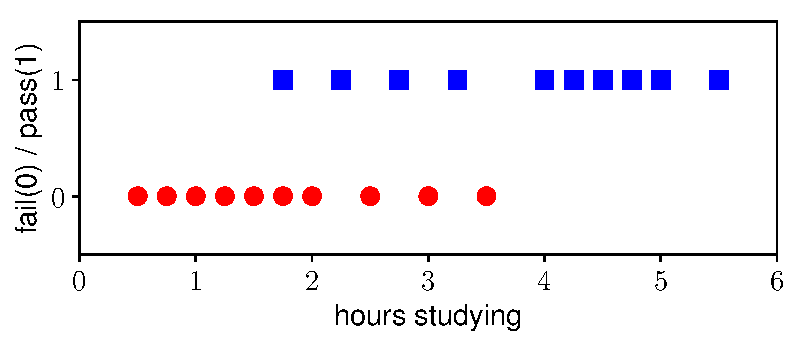
\includegraphics[width = \linewidth]{ex1.pdf}
\end{minipage} \hfill
\begin{minipage}[c]{0.5\linewidth}
    \caption{Ví dụ về kết quả thi dựa trên số giờ ôn tập. Trục hoành thể hiện thời gian ôn tập của mỗi sinh viên, trục tung gồm hai giá trị 0/fail (các điểm hình tròn) và 1/pass (các điểm hình vuông). Nguồn: machinelearningcoban.com 
}
    \label{fig13}
\end{minipage}
\end{figure}
\begin{figure}[ht!]
\begin{minipage}[c]{0.47\linewidth}
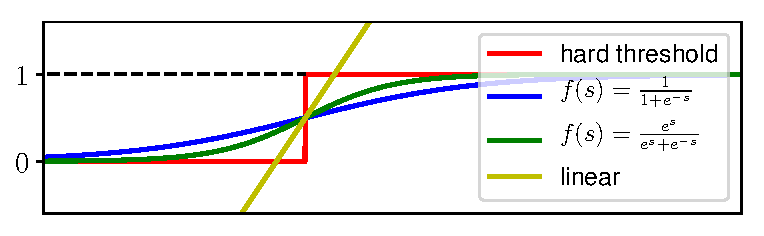
\includegraphics[width = \linewidth]{activation.pdf}
\end{minipage} \hfill
\begin{minipage}[c]{0.5\linewidth}
    \caption{Một vài ví dụ về các hàm kích hoạt khác nhau.  
}
    \label{fig14}
\end{minipage}
\end{figure}
\phantom{a}\\
Cùng nhìn vào hình \ref{fig14} ta thấy chỉ có hai hàm kích hoạt "khả thi" trong trường hợp của bài toán trên đó là hàm \textit{tanh} và hàm \textit{sigmoid}. Chúng có một vài tính chất quan trọng:
\begin{enumerate}
    \item Là các hàm số liên tục nhận giá trị thực, bị chặn trong khoảng (0,1).
    \item Nếu coi điểm có tung độ bằng 0.5 là ngưỡng, các điểm càng xa ngưỡng về phía bên trái có giá trị càng gần 0, các điểm càng xa ngưỡng về bên phải có giá trị càng gần một. Điều này phù hợp với nhận xét rằng càng học nhiều thì xác suất đỗ càng cao và ngược lại.
    \item Hai hàm này có đạo hàm mọi nơi, điều này có thể có ích trong tối ưu.
\end{enumerate}
\subsubsection*{Hàm mất mát - Loss Function}
Đối với các mô hình sử dụng biểu diễn xác suất cho các đầu ra, người ta thường chọn hàm mất mát là \textit{cross entropy loss}. \textit{cross entropy} cho biết mức độ khác biệt giữa hai phân bố xác suất. Ta sẽ chứng minh và phân tích kĩ hơn hàm mất mát này trong phần \textit{Hồi quy Softmax}.\\\\
\textit{Cross entropy} thường được dùng cho các bài toán phân loại đa lớp. Trong hồi quy logistic nếu đặt 
\begin{eqnarray} 
\label{eq17}
p(y_i=1|\textbf{x}_i;\textbf{w})  &=& a_i = f(\textbf{x}_i^{\text{T}}\textbf{w})  \\
\label{eq18}
p(y_i=0|\textbf{x}_i;\textbf{w}) &=& 1 - a_i =  1-f(\textbf{x}_i^{\text{T}}\textbf{w})
\end{eqnarray}
ta có \textit{cross entropy loss} cho hồi quy logistic:
\begin{equation}
    J(\textbf{w}) = -\frac{1}{N}\sum_{i=1}^{N} \left( y_i \log a_i + (1-y_i) \log (1-a_i) \right)
\end{equation}
Khi đó lấy gradient hai vế ta được:
\begin{equation}
    \nabla J(\textbf{w}) = -\frac{1}{N} \sum_{i=1}^{N} \left( \frac{y_i}{a_i} - \frac{1-y_i}{1-a_i} \right).f'(z_i)
    \label{eq20}
\end{equation}
Trong đó $z_i = \textbf{x}_i^{\text{T}}\textbf{w}$; $a_i = f(z_i)$. Nếu $f(s)$ là hàm sigmoid $\sigma(s)$ thì $\sigma'(s) = \sigma(s)(1-\sigma(s))$. Từ đây công thức (\ref{eq20}) trở thành:
\begin{equation}
    \nabla J(\textbf{w}) = -\frac{1}{N}\sum_{i=1}^{N}(y_i-a_i)\textbf{x}_i=-\frac{1}{N}\sum_{i=1}^{N}(y_i-\sigma(\textbf{x}_i^{\text{T}}\textbf{w}))\textbf{x}_i
    \label{eq21}
\end{equation}
Từ (\ref{eq21}) dễ suy ra công thức cập nhật SGD và mini-batch GD cho hồi quy logistic.
\\\\
\textbf{SGD}\\\\
Công thức cập nhật cho SGD như sau:
\begin{equation}
    \textbf{w} \leftarrow \textbf{w} + \eta. (y_i-\sigma(\textbf{x}_i^{\text{T}}\textbf{w}))\textbf{x}_i
    \label{eq22}
\end{equation}
\textbf{Mini-batch GD}\\\\
Công thức cập nhật cho Mini-batch GD như sau:
\begin{equation}
    \textbf{w} \leftarrow \textbf{w} - \eta. \frac{1}{N_b} \textbf{X}_{b}^{\text{T}}(\textbf{y}-\textbf{a})
    \label{eq23}
\end{equation}
Trong đó \textbf{y} là vector nhãn của các điểm dữ liệu trong mini-batch, \textbf{a} là vector đầu ra của các điểm dữ liệu trong mini-batch. \textbf{y} và \textbf{a} đều có kích thước $N_b\times1$\\\\
Trong bài này có vẻ sẽ tiện hơn nếu sử dụng SGD.
\begin{figure}[ht!]
    \centering
    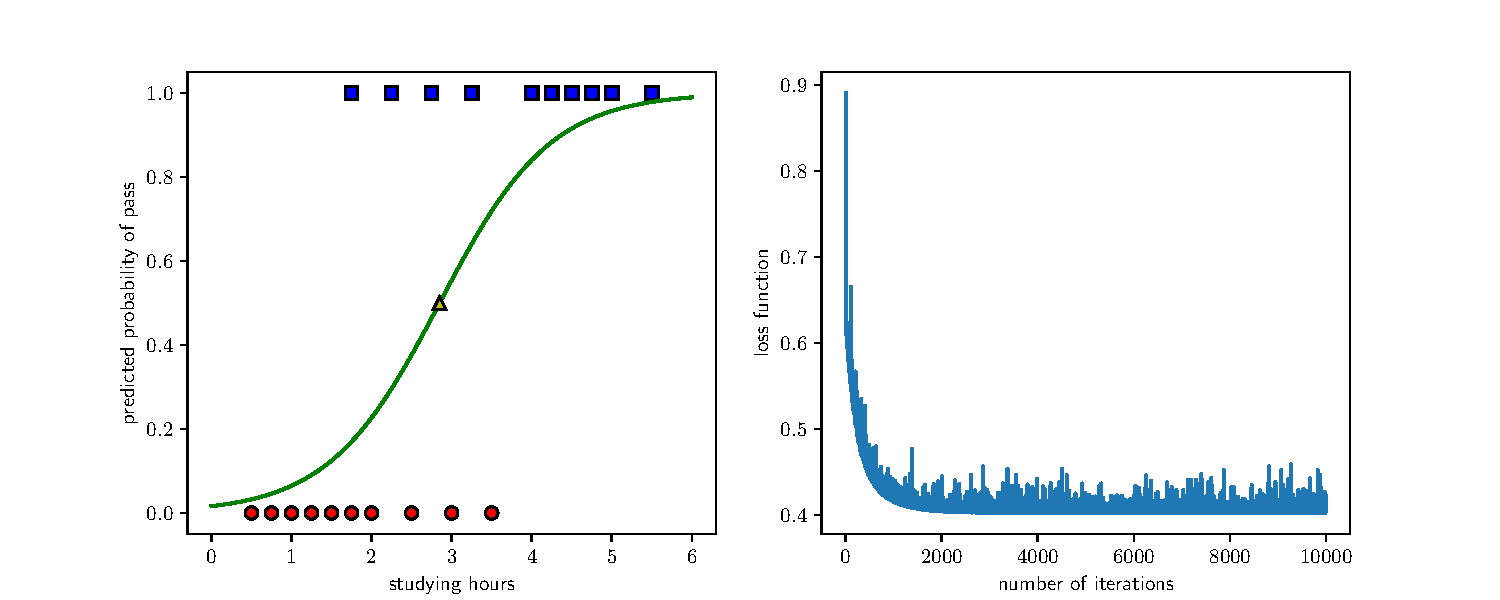
\includegraphics[width = 0.9\linewidth]{logistic_1d.pdf}
    \caption{Nghiệm cho ví dụ ở đầu bài ngưỡng: 0.5}
    \label{fig15}
\end{figure}

\begin{figure}[ht!]
    \centering
    \begin{subfigure}[b]{0.45\linewidth}
        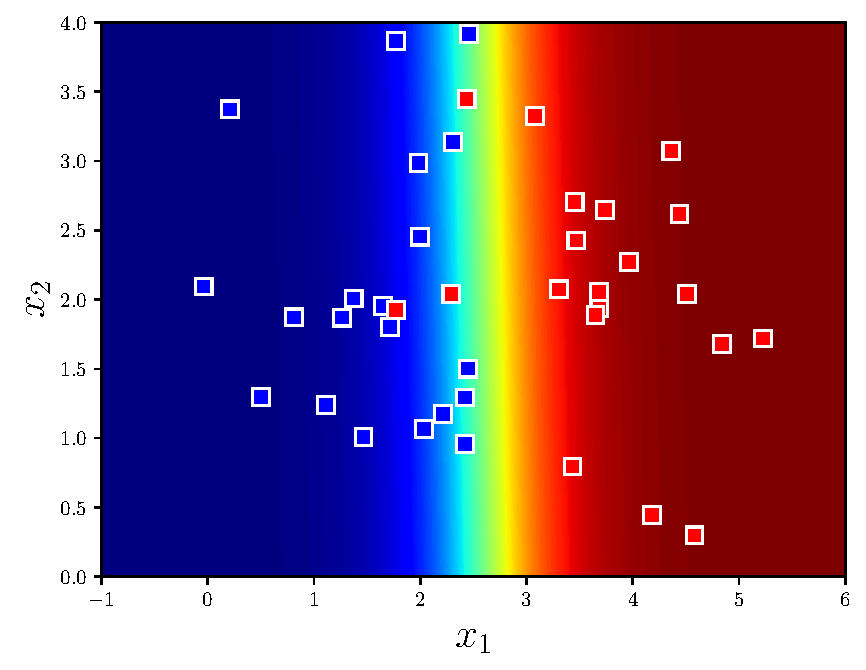
\includegraphics[width = \linewidth]{logistic_2d_3.pdf}
        \label{fig16a}
    \end{subfigure}
    \begin{subfigure}[b]{0.45\linewidth}
        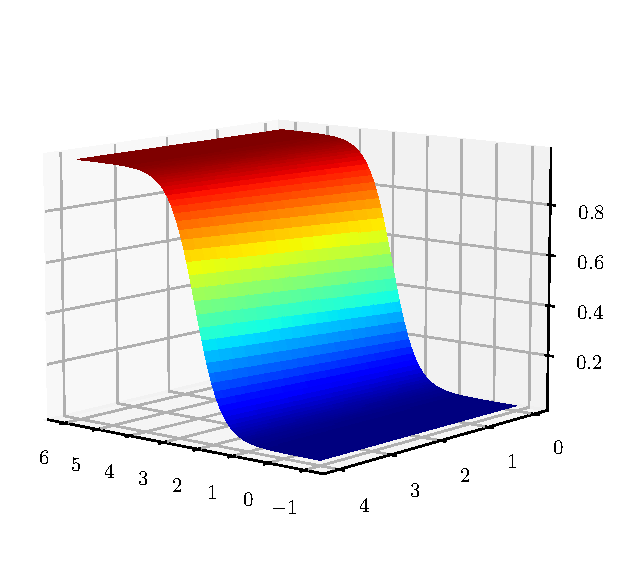
\includegraphics[width = \linewidth]{logistic_2d_4.pdf}
        \label{fig16b}
    \end{subfigure}
    \caption{Hồi quy logistic với dữ liệu hai chiều}
    \label{fig16}
\end{figure}
\phantom{a}\\
Hồi quy logistic đã khắc phục được nhược điểm của PLA. Tuy nhiên nếu để ý kĩ ta thấy rằng ranh giới của hồi quy logistic vẫn cơ bản là các đường tuyến tính (các siêu phẳng)! Điều này hoàn toàn có thể chứng minh như sau:\\\\
Giả sử những điểm có xác suất đầu ra lớn hơn 0.5 được gán nhãn 1. Tập hợp các điểm này là nghiệm của bất phương trình:
$$P(y=1|\textbf{x};\textbf{w})>0.5 \Leftrightarrow \frac{1}{1+e^{-\textbf{x}^{\text{T}}\textbf{w}}}>0.5 \Leftrightarrow e^{-\textbf{x}^{\text{T}}\textbf{w}}<1\Leftrightarrow \textbf{x}^{\text{T}}\textbf{w}>0$$
Tương tự với các điểm có nhãn 0. Suy ra ranh giới giữa hai nhãn là siêu phẳng $\textbf{x}^{\text{T}}\textbf{w}=0$
\subsection{Hồi quy Softmax}
Các bài toán phân loại trong thực tế thường có nhiều lớp dữ liệu. Tức ở tầng đầu ra có nhiều hơn 2 nút, mặc dù ta vẫn có thể sử dụng các bộ phân loại nhị phân cho các bài toán phân loại đa lớp tuy nhiên chúng đều có những nhược điểm lớn. Trong bài này, một mô hình tuyến tính sẽ khắc phục những nhược điểm đó, là mở rộng của mô hình hồi quy logistic, \textit{hồi quy Softmax}. Cũng giống như hồi quy logistic cụm từ "hồi quy" chỉ mang tính lịch sử, hồi quy Softmax thường được sử dụng cho các bài toán phân loại. Hồi quy Softmax là một trong những thành phần phổ biến nhất trong các bộ phân loại hiện nay.
\subsubsection*{Hàm softmax}
Để xây dựng từ đầu cho hồi quy Softmax chắc ta phải đi từ \textit{phân loại đa lớp với hồi quy logistic}. Tuy nhiên do hạn chế về mặt thời gian và điều đó cũng không quá quan trọng, ta có thể nhìn dưới một góc độ khác, góc độ này là do bản thân tôi cảm nhận. Đó là mô hình hồi quy Softmax, giống như mô hình \textit{công thức xác suất đầy đủ} và \textit{công thức Bayes}.\\\\
Một thực tế đơn giản như sau, trong các mô hình tuyến tính đơn giản phía trước, bộ tham số của ta chỉ là một vector với một điểm dữ liệu đầu ra. Một cách rất tự nhiên, ta hoàn toàn có thể tăng số lượng tham số ấy lên để có được nhiều đầu ra. Sau đó so sánh kết quả giữa chúng và dự đoán lớp của dữ liệu đang xử lí! Đó là ý tưởng của hồi quy logistic cho phân loại đa lớp.\\\\
Tuy nhiên cách làm trên có nhược điểm rằng, đó là giữa các điểm đầu ra, không có ràng buộc với nhau. Tức không thể kết luận một cách đơn giản và trực quan rằng đầu ra nút này cao hơn thì sẽ chính xác hơn, mặc dù điểu đấy rất hợp lí. Do đó hồi quy Softmax, theo tôi thì dựa trên ý tưởng của \textit{Công thức xác suất đầy đủ}. Điều đấy có nghĩa rằng, tổng xác suất của điểm dữ liệu vào các lớp phải bằng 1.\\\\
Hàm Softmax được cho như sau:
\begin{equation}
    a_i = \frac{\exp(z_i)}{\sum_{j=1}^{C}\exp(z_j)}, \forall i = 1,2,\ldots,C.
    \label{eq24}
\end{equation}
Công thức (\ref{eq24}) có các đặc điểm sau:
\begin{enumerate}
    \item $z_i = \textbf{x}^{\text{T}}\textbf{w}_i$ càng lớn thì xác suất dữ liệu rơi vào lớp thứ i càng cao.
    \item Đầu ra $a_i$ dương, có tổng bằng một và giữ được thứ tự của $z_i$
\end{enumerate}
\begin{figure}[ht!]
    \centering
    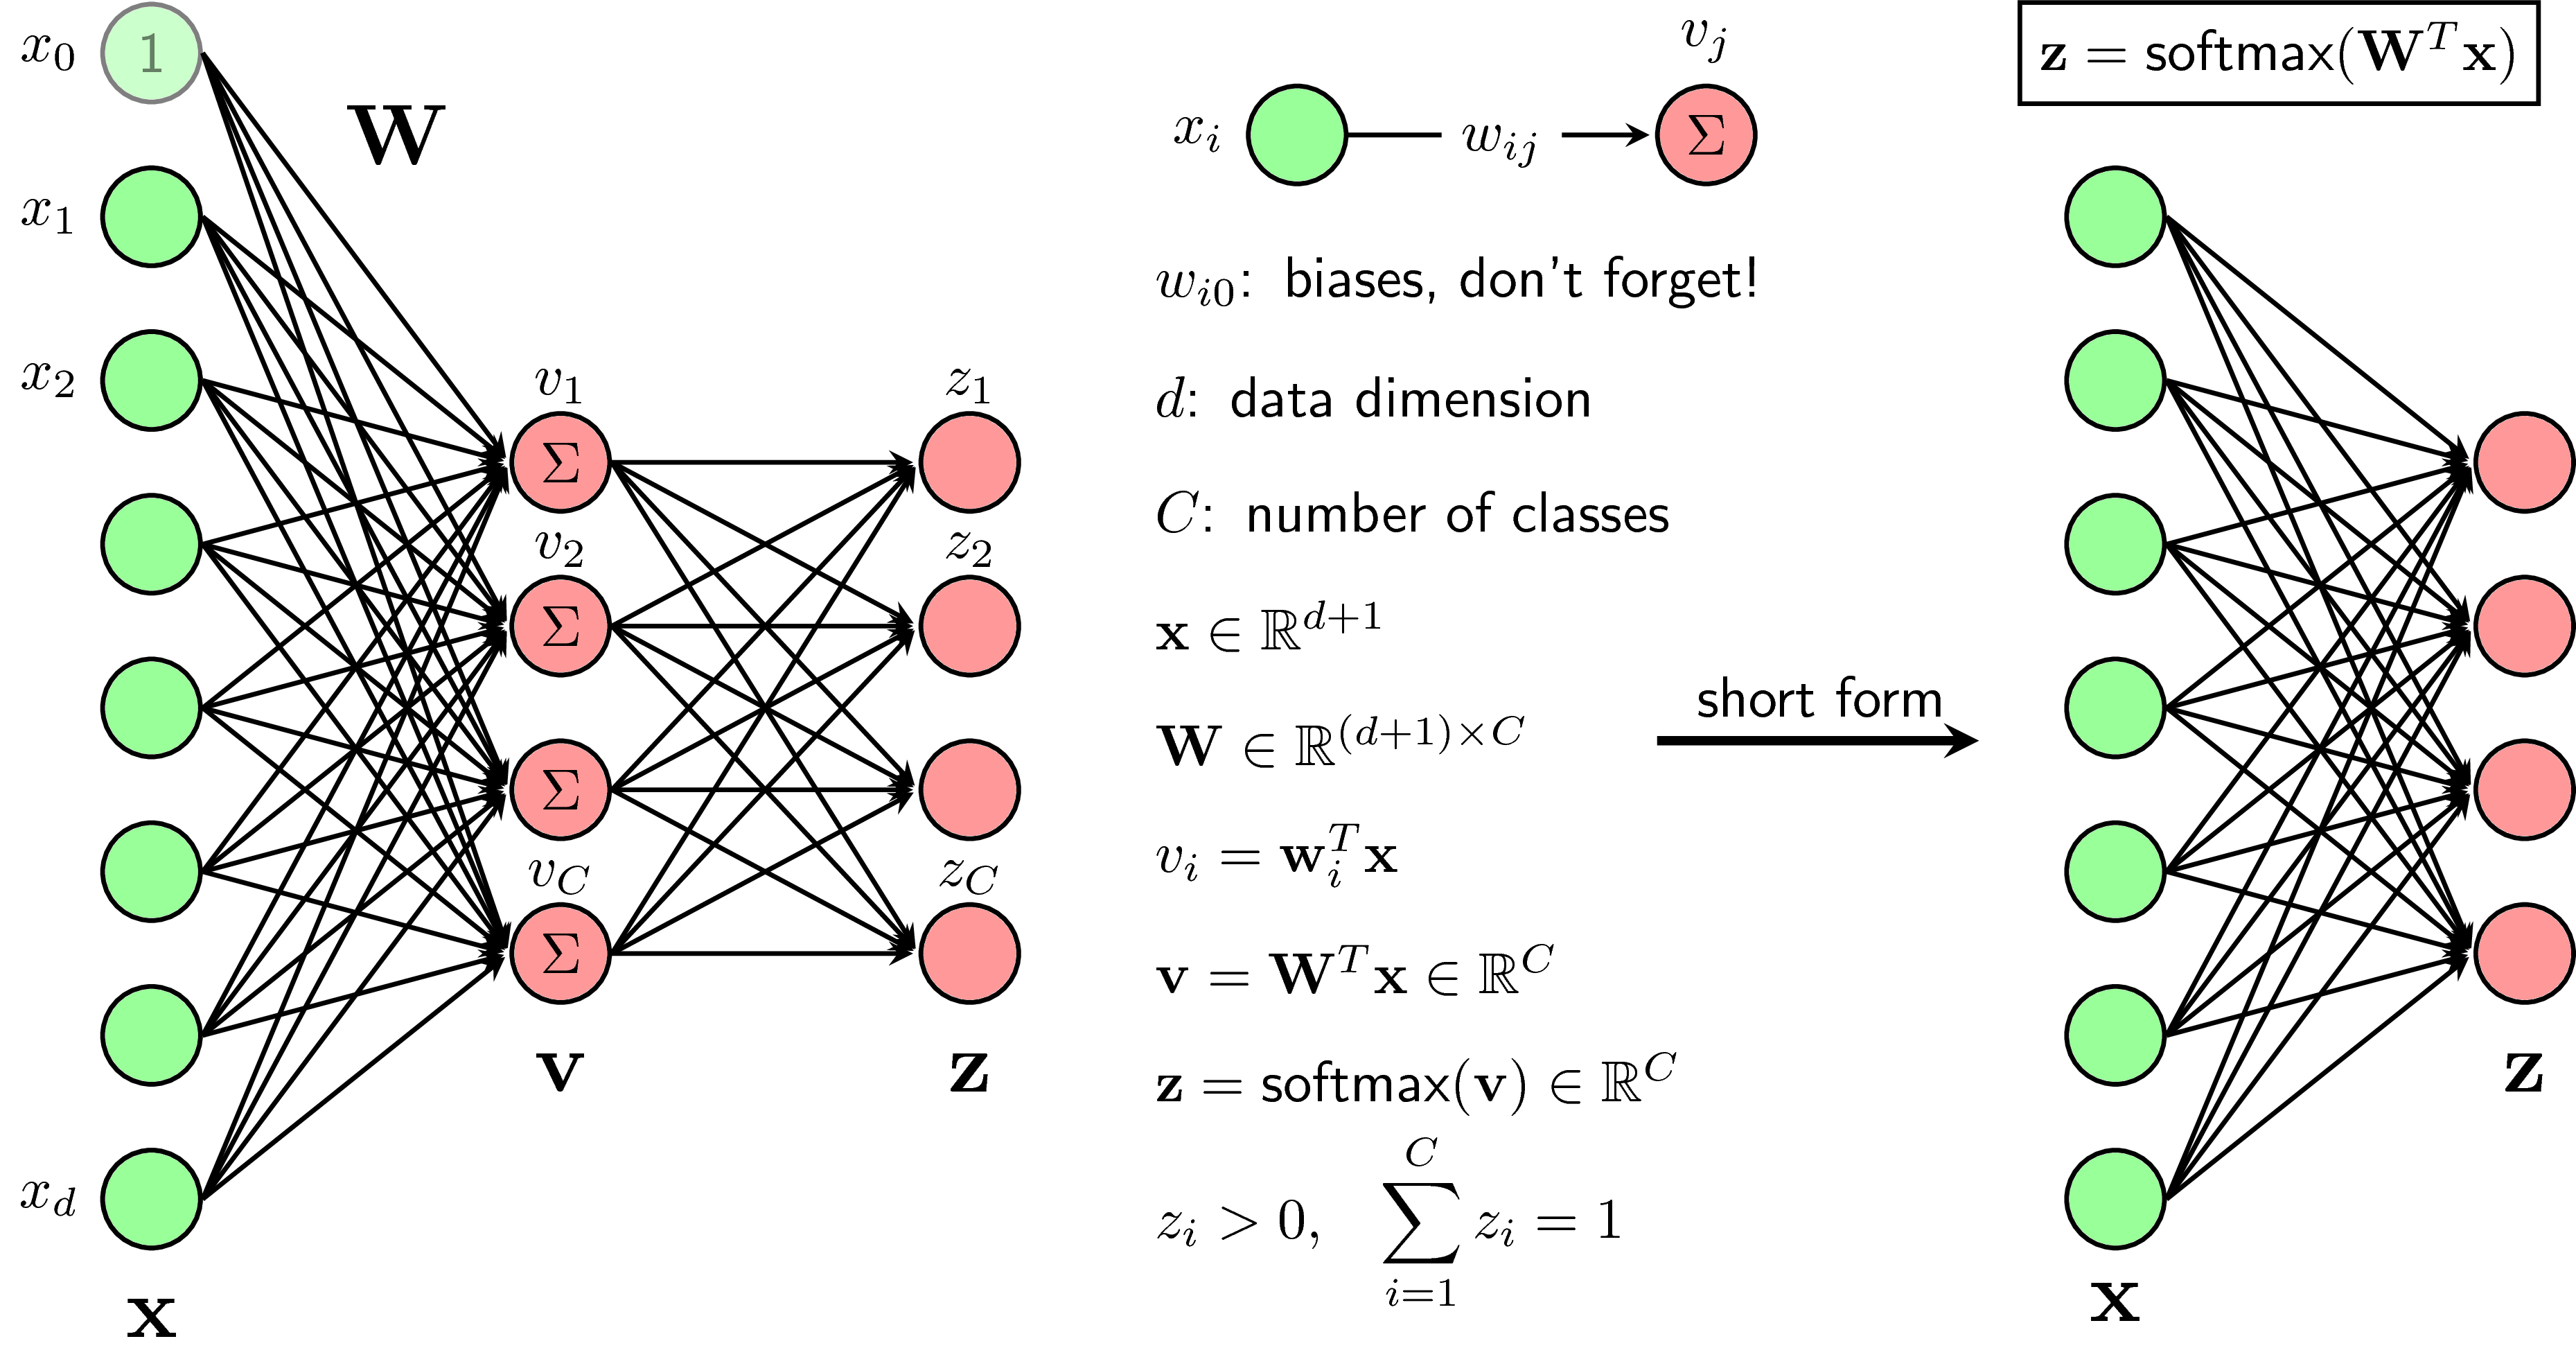
\includegraphics[width = \linewidth]{softmax.png}
    \caption{Mô hình hồi quy softmax dưới dạng neural network. Nguồn: machinelearningcoban.com}
    \label{fig17}
\end{figure}
\subsubsection*{Hàm softmax phiên bản ổn định}
$\exp(x)$ có nhiều ưu điểm như đồng biến, luôn dương. Tuy nhiên nó cũng có một nhược điểm lớn, đó là khi một trong các $z_i$ quá lớn, việc tính toán $\exp(z_i)$ có thể gây ra hiện tượng tràn số, ảnh hưởng tới kết quả của hàm softmax. Dể khắc phục tình trạng này có thể làm như sau:
\begin{equation}
    \frac{\exp(z_i)}{\sum_{j=1}^{C}\exp(z_j)}=\frac{\exp(-c)\exp(z_i)}{\exp(-c)\sum_{j=1}^{C}\exp(z_j)} = \frac{\exp(z_i-c)}{\sum_{j=1}^{C}\exp(z_j-c)}
    \label{eq25}
\end{equation}
$c$ là một hằng số bất kì. Trong thực tế, $c$ thường được chọn $c = \text{max} z_i$
\subsubsection*{Hàm mất mát - Loss Function}
Như đã giới thiệu qua ở phần hồi quy logistic, hàm mất mát thường được sử dụng cho các bài toán phân loại sử dụng xác suất là \textit{Cross entropy loss}.\\\\
Giả sử điểm dữ liệu $\textbf{x}_i$ có nhãn dưới dạng one hot là $\textbf{y}_i,\text{ } \sum_{j=1}^{C}=1, \text{ } \forall\text{ }  y_{ij} \geq 0$\\\\
Xác suất để một điểm dữ liệu rơi vào nhãn $\textbf{y}_i$ là:
\begin{equation}
    P(\textbf{y}_i|\textbf{x}_i,\textbf{W}) = \prod_{j=1}^{C}a_{ij}^{y_{ij}}
    \label{eq26}
\end{equation}
Hiển nhiên ta muốn đạt cực đại vế phải trong công thức trên. Lấy $-$ loga hai vế. Ta có công thức của \textit{Cross entropy loss}:
\begin{equation}
    J_i(\textbf{W}) = -\log(\prod_{j=1}^{C}a_{ij}^{y_{ij}}) = -\sum_{j=1}^{C}y_{ij}\log{a_{ij}}
    \label{eq27}
\end{equation}
Hàm mất mát cho trên toàn tập dữ liệu:
\begin{equation}
    J(\textbf{W}) = -\frac{1}{N}\sum_{i=1}^{N}\sum_{j=1}^{C}y_{ij}\log{a_{ij}}
    \label{eq28}
\end{equation}
Lấy gradident hai vế ta được như sau:
\begin{equation}
    \nabla J(\textbf{W}) = -\frac{1}{N}\sum_{i=1}^{N}\nabla J_i(\textbf{W})
\end{equation}
Mà 
\begin{equation}
    \nabla J(\textbf{W}) = [\nabla_{\textbf{w}_1}J_i, \nabla_{\textbf{w}_2}J_i,\ldots,\nabla_{\textbf{w}_C}J_i]
\end{equation}
Do đó ta chỉ cần tính $\nabla_{\textbf{w}_k}J_i$ sau đó thay vào các công thức trên ta sẽ ra được công thức cập nhật cho cả SGD và mini-batch SGD.\\\\
Ta có
\begin{eqnarray} 
\label{eq31}
\nabla_{\textbf{w}_k}J_i &=& \nabla_{\textbf{w}_k} \left( -\sum_{j=1}^{C}y_{ij}\log{\frac{\exp(z_{ị})}{\sum_{j=1}^{C}\exp(z_{ij})}} \right)  \\
\label{eq32}
&=& \nabla_{\textbf{w}_k} \left( -\sum_{j=1}^{C}y_{ij} \left( z_{ij} - \log(\sum_{j=1}^{C}\exp(z_{ij})) \right) \right)\\
&=& -y_{ik}\textbf{x}_i + \left(\sum_{j=1}^{C}y_{ij}\right).\frac{\exp(z_{ik})}{\sum_{j=1}^{C}\exp(z_{ij})}\textbf{x}_i\\
 \label{eq33}
 &=& -y_{ik}\textbf{x}_{i}+a_{ik}\textbf{x}_i\\
 \label{eq34}
 &=& (a_{ik}-y_{ik})\textbf{x}_i\\
 \label{eq35}
 &=& \textbf{x}_i.\textbf{e}_{i}^{\text{T}}
\end{eqnarray}
Trong đó $\textbf{e}_i = \textbf{a}_i - \textbf{y}_i$, suy ra $\nabla J$:
\begin{equation}
    \nabla J = \frac{1}{N}\textbf{X}^{\text{T}}\textbf{E}
    \label{eq37}
\end{equation}
Từ hai công thức (\ref{eq35}) và (\ref{eq37}) ta suy ra công thức cập nhật cho hồi quy Softmax:\\\\
\textbf{SGD}\\\\
Công thức cập nhật cho SGD như sau:
\begin{equation}
    \textbf{W} \leftarrow \textbf{W} - \eta.\textbf{x}_i\textbf{e}_i^{\text{T}}
    \label{eq38}
\end{equation}
\textbf{Mini-batch GD}\\\\
Công thức cập nhật cho Mini-batch GD như sau:
\begin{equation}
    \textbf{W} \leftarrow \textbf{W} - \frac{\eta}{N_b} \textbf{X}_{b}^{\text{T}}\textbf{E}_{b}
\end{equation}
\subsection{Mạng neuron đa tầng và lan truyền ngược}
Một mạng neuron trong thực tế rất phức tạp có tới hàng triệu tham số. Bên cạnh hai tầng đầu, ra thì còn có thêm các tầng ẩn/tầng trung gian để tăng khả năng học của mô hình. Đây là một phần phức tạp, do hạn chế về thời gian và tự chủ về hình ảnh,\ldots Tôi không thể làm quá sâu vào lúc này, nên ta sẽ chỉ điểm qua những điểm chính nhất!
\subsubsection{Các kí hiệu và khái niệm}
\subsubsection*{Tầng}
Như đã giới thiệu ở trên, một mạng neuron đa tầng có thể có nhiều tầng ẩn (hidden layer) ở giữa tầng đầu vào và tầng đầu ra.\\\\
Số lượng tầng trong một mạng neuron đa tầng được kí hiệu là $L$, được tính bằng số tầng ẩn cộng một. Khi đếm số tầng của một mạng neuron đa tầng, ta không tính tầng đầu vào.
\subsubsection*{Nút}
Mỗi điểm hình tròn (Hình \ref{fig18}) trong một tầng được gọi là một \textit{nút} (node hoặc unit). Đầu vào của tầng ẩn thứ \textit{l} được kí hiệu bởi $\textbf{z}^{(l)}$, đầu ra tại mỗi tầng thường được kí hiệu là $\textbf{a}^{(l)}$ (thể hiện \textit{activation}, tức giá trị tại các nút sau khi áp dụng hàm kích hoạt lên đầu vào $\textbf{z}^{(l)}$). 
\begin{figure}[ht!]
\begin{minipage}[c]{0.57\linewidth}
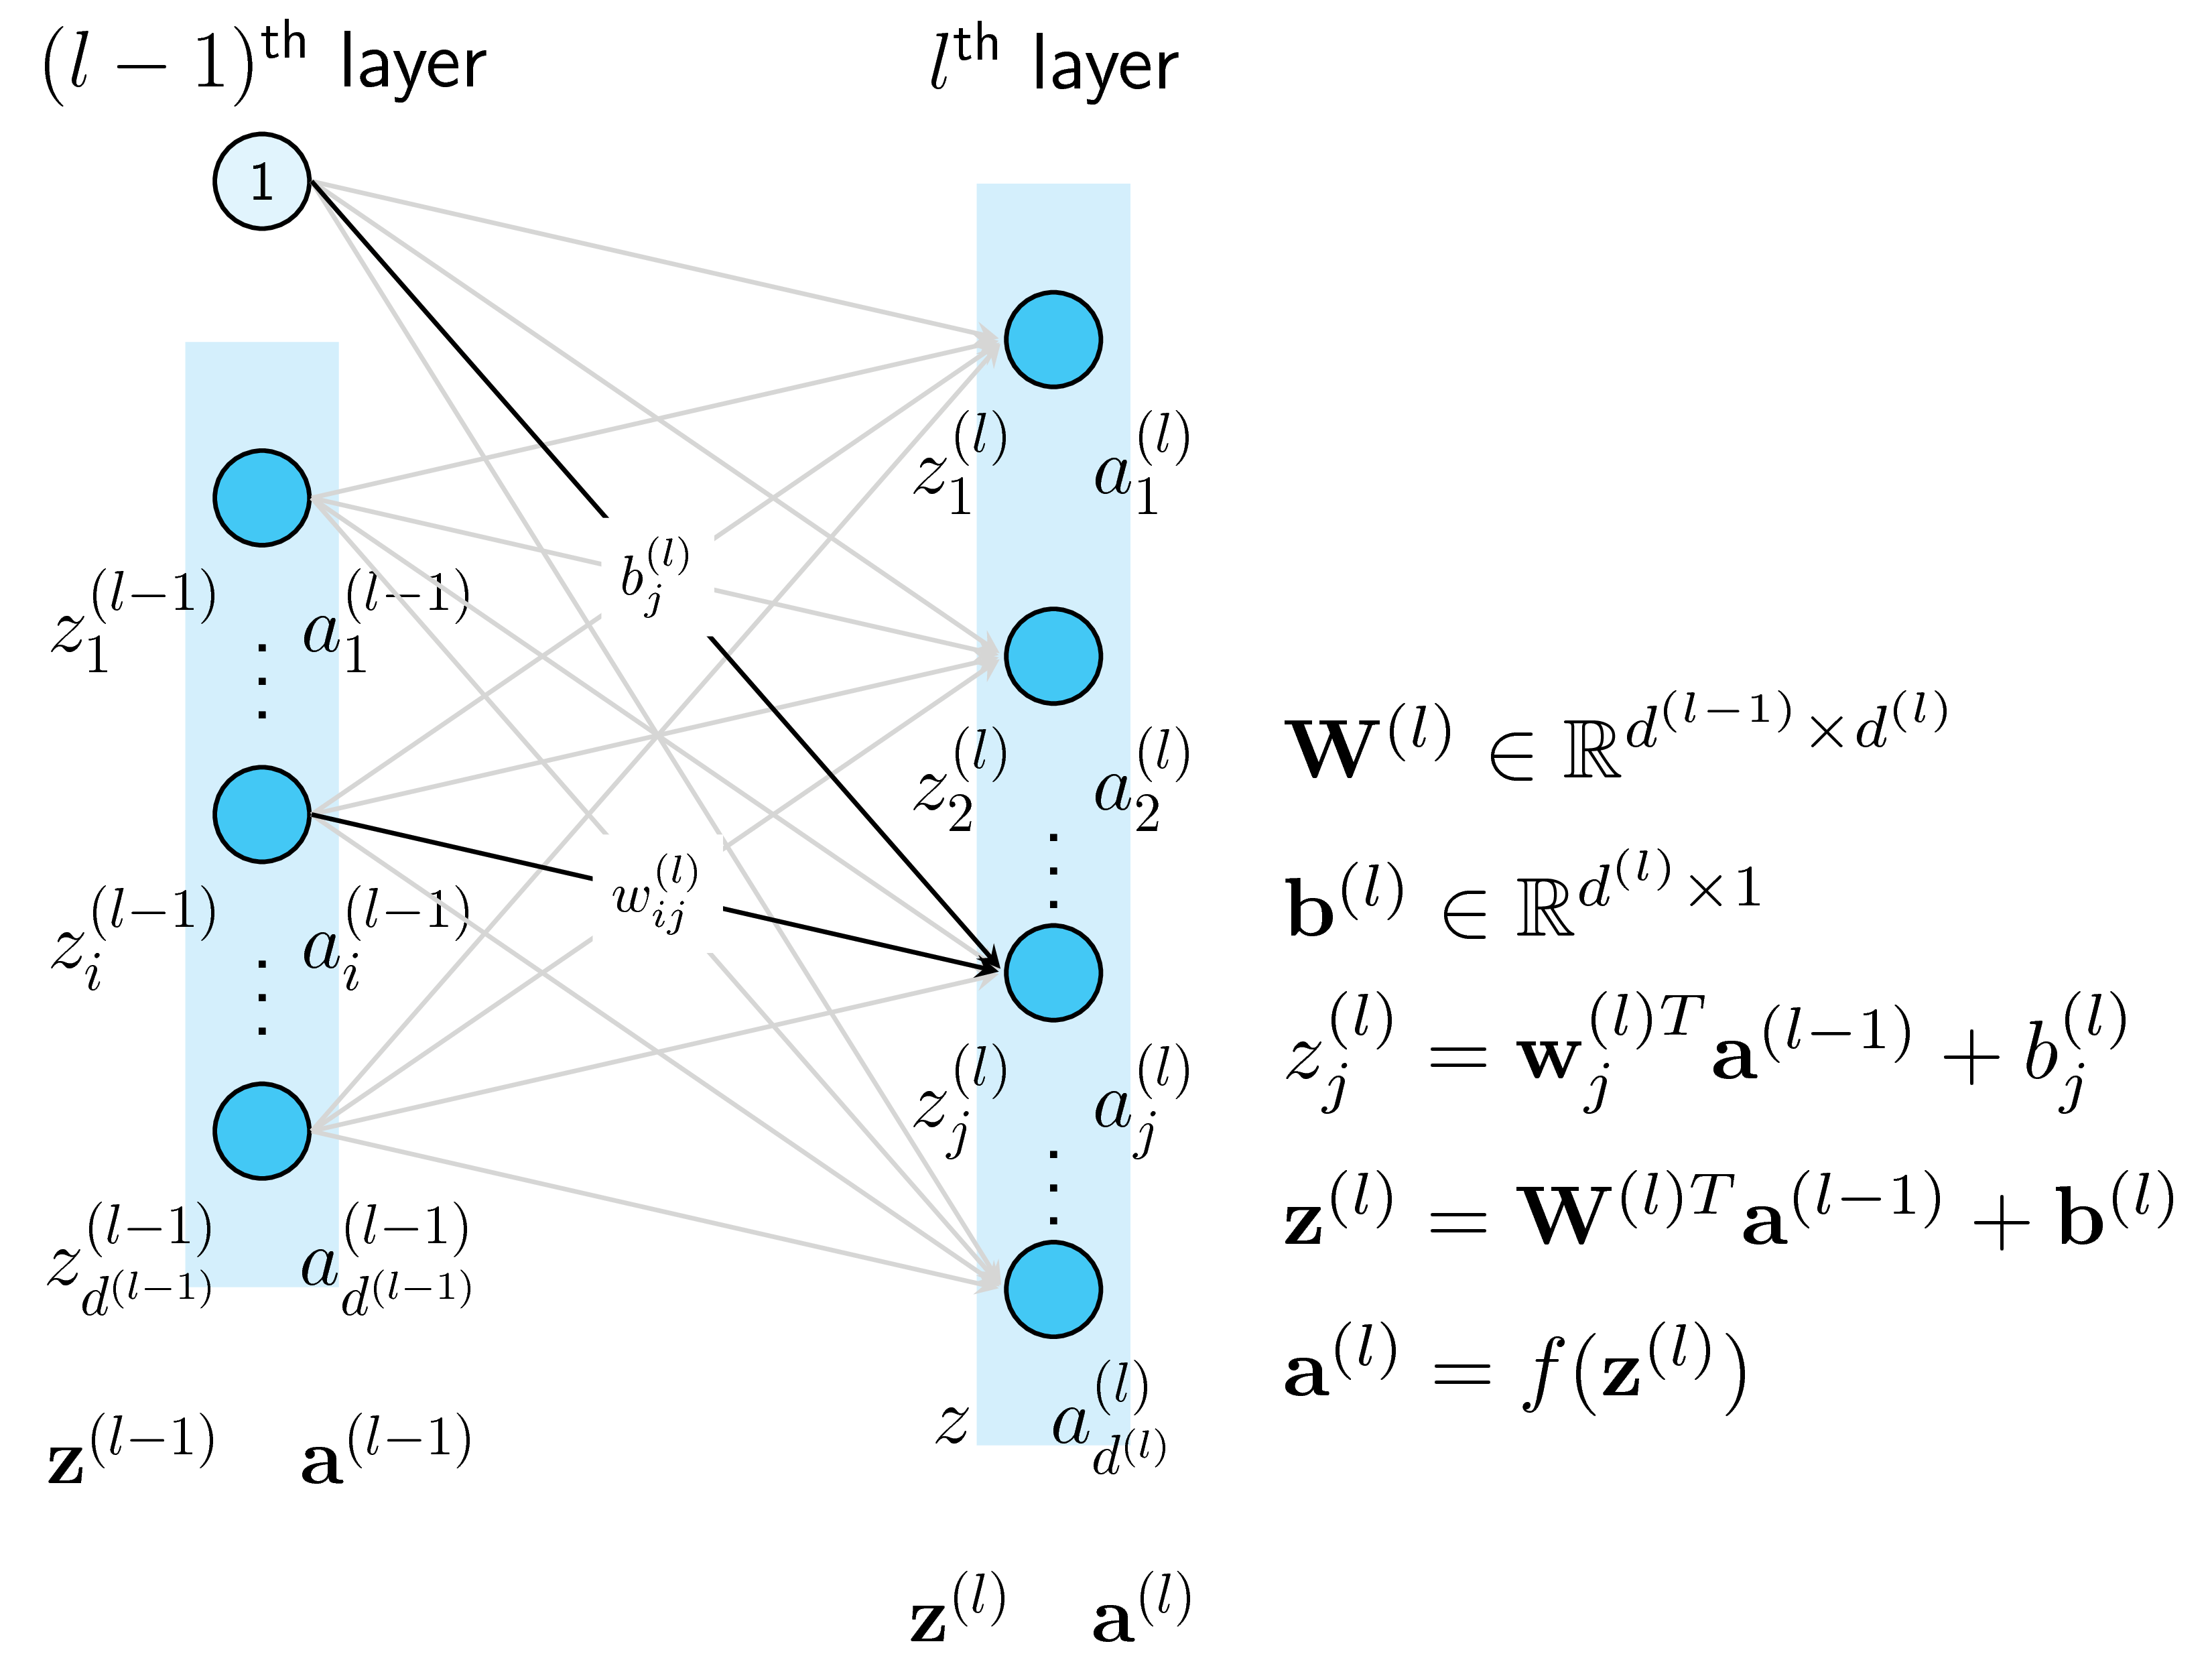
\includegraphics[width = \linewidth]{mlp_notation.png}
\end{minipage} \hfill
\begin{minipage}[c]{0.4\linewidth}
    \caption{Các kí hiệu sử dụng trong mạng neuron đa tầng. nguồn: machinelearningcoban.com  
}
    \label{fig18}
\end{minipage}
\end{figure}

\subsubsection*{Trọng số và hệ số điều chỉnh}
Có \textit{L} ma trận trọng số cho một mạng neuron có \textit{L} tầng. Các ma trận này được kí hiệu là $\textbf{W}^{(l)} \in \mathbb{R}^{d^{(l-1)}\times d^{(l)}}$, $l = 1,2,\ldots, L$ trong đó $\textbf{W}^{(l)}$ thể hiện các kết nối từ tầng thứ $l-1$ tới tầng thứ $l$ (giả sử tầng đầu vào là tầng 0). Các hệ số điều chỉnh của tầng thứ ($l$) được kí hiệu là $\textbf{b}^{(l)} \in \mathbb{R}^{d^{(l)}}$. Xem hình \ref{fig18}. Khi tối ưu một mạng neuron đa tầng, nhiệm vụ của ta là đi tìm các trọng số và hệ số điều chỉnh này!
\subsubsection{Hàm kích hoạt}
Như đã giới thiệu trong hồi quy logistic, ta có hai hàm kích hoạt khá mềm mại, đạo hàm khá đơn giản là sigmoid và tanh. Tuy nhiên trong các mạng neuron đa tầng người ta sẽ ít dùng hai hàm này, thường chỉ được dùng ở các tầng đầu ra điều này do hiện tượng \textit{tiêu biến gradient } (gradient vanishing). Tức là càng đi sâu vào mạng, đạo hàm của nó gần như bằng 0, do đó việc cập nhật bằng GD dường như là vô ích! Do đó người ta thường dùng hàm khác để thay thế, đơn giản hơn và đặc biết là khắc phục được điều này, đó là hàm ReLU! Hàm này là một trong những nhân tố đã góp phần làm nên sự bùng nổ của AI, Machine Learning nói chung và Deep Learning, Thị giác máy tính nói riêng! Biểu thức của ReLU rất đơn giản như sau:
\begin{equation}
    \text{ReLU} = \text{max}(0, z)
    \label{eq40}
\end{equation}
\subsubsection{Lan truyền ngược}
Như đã nói ở phía trên, nhiệm vụ của chúng ta là đi tìm các trọng số $\textbf{W}^{(l)}$ và $\textbf{b}^{(l)}$. Hiển nhiên ta sẽ tìm thông qua GD, tuy nhiên để làm được điều này ta phải tính được gradient của hàm mất mát theo từng ma trận trọng số $\textbf{W}^{(l)}$ và vector điều chỉnh $\textbf{b}^{(l)}$.\\\\
Để làm được điều này ta cần thông qua hai bước sau:
\begin{enumerate}
    \item Lan truyền thuận. Tính, lưu lại tất cả các biến trung gian.
    \item Lan truyền ngược. Sử dụng quy tắc chuỗi (chain rule) trong giải tích, để tìm ra gradient tại vị trí mong muốn theo chiều ngược bắt đầu từ tầng cuối!
\end{enumerate}
\subsubsection*{Lan truyền thuận}
Quá trình lan truyền thuận được mô tả như sau:
\begin{eqnarray}
\label{eq41}
    \textbf{a}^{(0)} &=& \textbf{x}\\
    \label{eq42}
    \textbf{z}^{(l)} &=& \textbf{W}^{(l)}\textbf{a}^{(l-1)}+\textbf{b}^{(l)}, l=1,2,\ldots,L\\
    \label{eq43}
    \textbf{a}^{(l)} &=& f^{(l)}(\textbf{z}^{(l)}), l=1,2,\ldots,L\\
    \label{eq44}
    \hat{\textbf{y}} &=& \textbf{a}^{(L)}
\end{eqnarray}
với $N$ là số cặp dữ liệu $(\mathbf{x}, \mathbf{y})$ trong tập huấn luyện. Theo
các công thức này, việc tính toán trực tiếp các giá trị gradient tương đối phức
tạp vì hàm mất mát không phụ thuộc trực tiếp vào các ma trận trọng số và vector
điều chỉnh. Phương pháp phổ biến nhất được dùng có tên là \textit{lan truyền ngược}
(backpropagation) giúp tính gradient ngược từ tầng cuối cùng đến tầng đầu tiên.
Tầng cuối cùng được tính toán trước vì nó ảnh hưởng trực tiếp tới {đầu ra dự
đoán} và hàm mất mát. Việc tính toán gradient của các ma trận trọng số trong các
tầng trước được thực hiện dựa trên quy tắc chuỗi quen thuộc cho {gradient của hàm
hợp}.\\\\
Stochastic gradient descent có thể được sử dụng để cập nhật các ma trận trọng số và vector điều chỉnh dựa trên một cặp điểm huấn luyện $\mathbf{x, y}$. Đơn giản hơn, ta coi $J$ là hàm mất mát nếu chỉ xét cặp điểm này.
Đạo hàm riêng của hàm mất mát theo \textit{chỉ một thành phần} của ma trận trọng số
của tầng đầu ra:
\begin{eqnarray}
\frac{\partial J}{\partial w_{ij}^{(L)}} &=& \frac{\partial J}{\partial
z_j^{(L)}}. \frac{\partial z_j^{(L)}}{\partial w_{ij}^{(L)}} = e_j^{(L)} a_i^{(L-1)}
\end{eqnarray}
trong đó $\displaystyle e_j^{(L)} = \frac{\partial J}{\partial z_j^{(L)}} $
thường là một đại
lượng {không quá khó để tính toán} và $\displaystyle\frac{\partial
z_j^{(L)}}{\partial w_{ij}^{(L)}}  = a_i^{(L-1)}$ vì $z_j^{(L)} = \mathbf{w}_j^{(L)T}\mathbf{a}^{(L-1)} + b_j^{(L)}$.
Tương tự, gradient của hàm mất mát theo hệ số tự do của tầng cuối cùng là
\begin{equation}
\frac{\partial J}{\partial b_{j}^{(L)}} = \frac{\partial J}{\partial z_j^{(L)}}. \frac{\partial z_j^{(L)}}{\partial b_{j}^{(L)}} = e_j^{(L)}
\end{equation}
Với đạo hàm riêng theo trọng số ở các tầng $l < L$, hãy quan sát Hình
\ref{fig19}. Ở đây, tại mỗi nút, đầu vào $z$ và đầu ra $a$ được viết
riêng để tiện theo dõi.
\begin{figure}[ht!]
    \centering
    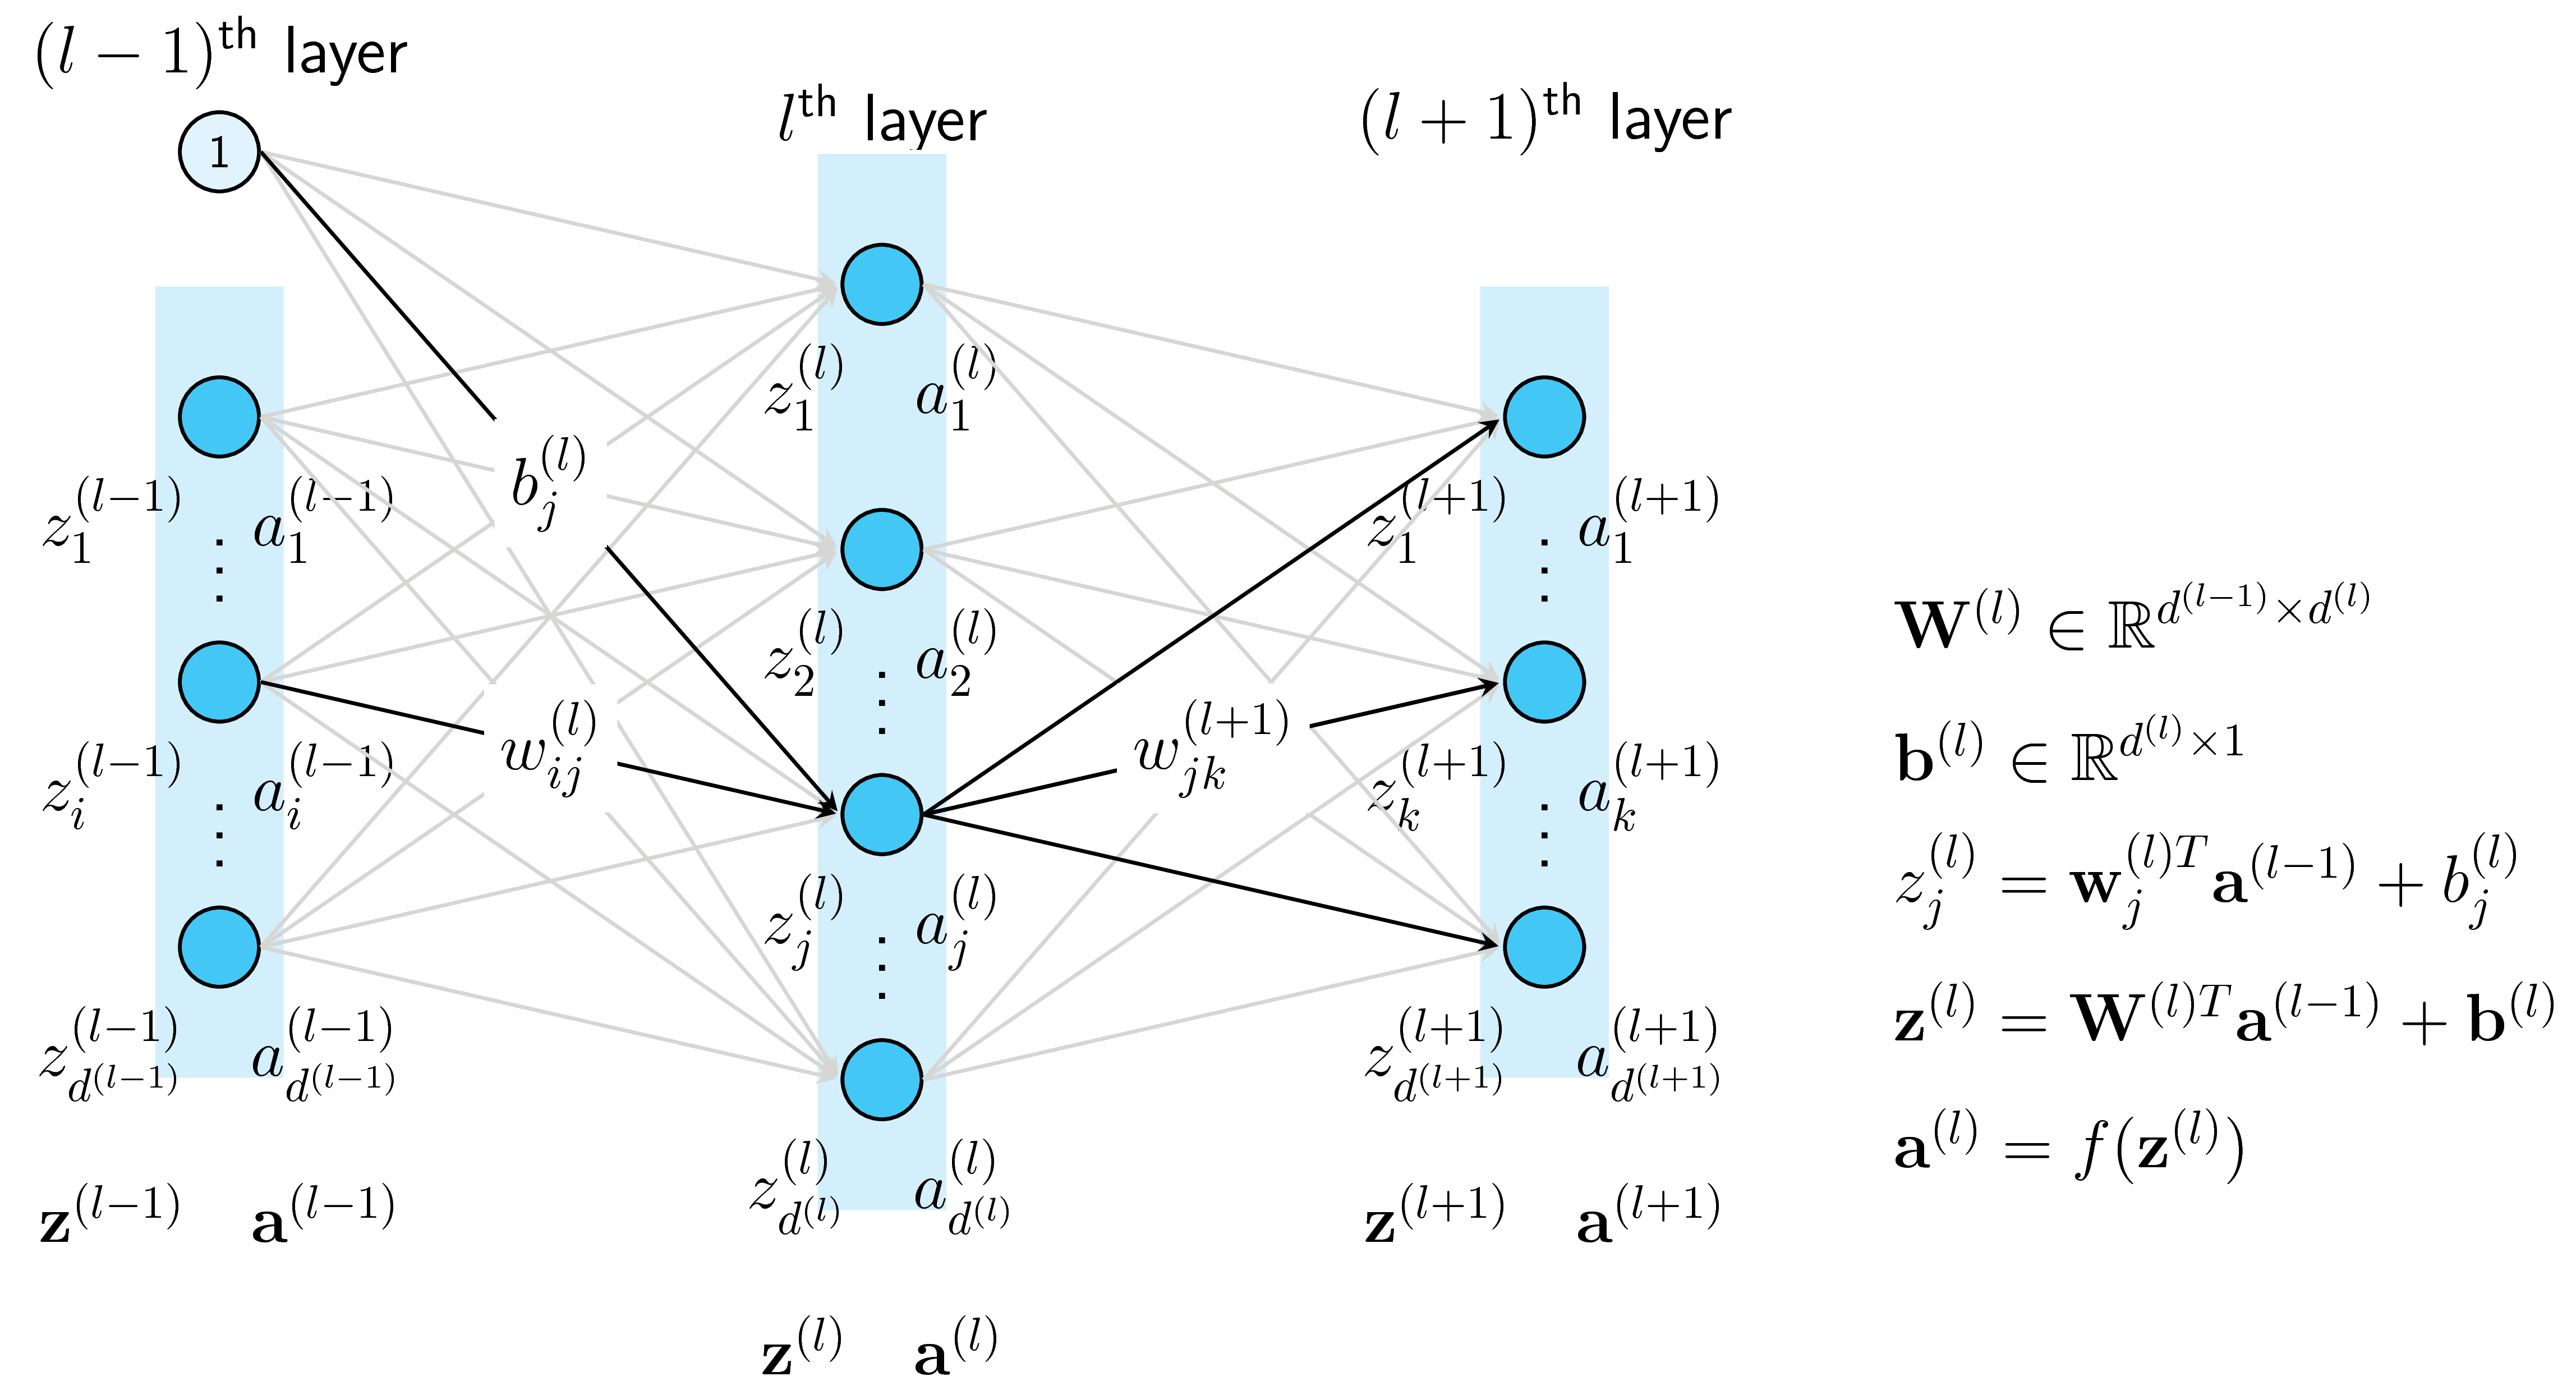
\includegraphics[width = \linewidth]{backpropagation.png}
    \caption{Mô phỏng cách tính lan truyền ngược. Tầng cuối có thể là tầng đầu ra. nguồn: machinelearningcoban.com}
    \label{fig19}
\end{figure}
\\\\
Dựa vào Hình \ref{fig19}, bằng quy nạp ngược từ cuối, ta có thể tính được:
\begin{eqnarray}
\frac{\partial J}{\partial w_{ij}^{(l)}} &=& \frac{\partial J}{\partial
z_j^{(l)}}. \frac{\partial z_j^{(l)}}{\partial w_{ij}^{(l)}} = e_j^{(l)} a_i^{(l-1)}.
\end{eqnarray}
với:
\begin{eqnarray*}
e_j^{(l)} &=& \frac{\partial J}{\partial z_j^{(l)}} = \frac{\partial J}{\partial a_j^{(l)}} . \frac{\partial a_j^{(l)}}{\partial z_j^{(l)}} \\\
&=& \left( \sum_{k = 1}^{d^{(l+1)}} \frac{\partial J}{\partial z_k^{(l+1)}}
.\frac{\partial z_k^{(l+1)}}{\partial a_j^{(l)}} \right) f^{(l)'}(z_j^{(l)}) =\left( \sum_{k = 1}^{d^{(l+1)}} e_k^{(l+1)} w_{jk}^{(l+1)} \right)
f^{(l)'}(z_j^{(l)}) \\
&=& \left(\textbf{w}_{j:}^{(l+1)}\textbf{e}^{(l+1)}f^{(l)'}\right)(z_j^{(l)})
\end{eqnarray*}
trong đó $\mathbf{e}^{(l+1)} = [e_1^{(l+1)}, e_2^{(l+1)}, ...,
e_{d^{(l+1)}}^{(l+1)}]^T \in \mathbb{R}^{d^{(l+1)}\times 1} $ và
$\mathbf{w}_{j:}^{(l+1)}$ được hiểu là \textbf{hàng} thứ $j$ của ma trận
$\mathbf{W}^{(l+1)}$ (chú ý dấu hai chấm, khi không có dấu này, chúng ta mặc
định dùng nó để ký hiệu cho vector \textit{cột}).
Dấu $\sum$ tính tổng ở dòng thứ hai trong phép tính trên xuất hiện vì
$a_{j}^{(l)}$ {đóng góp} vào việc tính tất cả các $z_k^{(l+1)}, k = 1, 2,
\dots, d^{(l+1)}$. Biểu thức đạo hàm ngoài dấu ngoặc lớn xuất hiện vì $a_j^{(l)}  =
f^{(l)}(z_j^{(l)})$. Tới đây, ta có thể thấy rằng việc hàm kích hoạt có
đạo hàm đơn giản sẽ có ích rất nhiều trong việc tính toán.Với cách làm tương tự, bạn đọc có thể suy ra
\begin{equation}
\frac{\partial J}{\partial b_j^{(l)}} = e_j^{(l)}.
\end{equation}
Nhận thấy rằng trong những công thức trên, việc tính các $e_j^{(l)}$ đóng một vài trò quan trọng. Hơn nữa, để tính được giá trị này, ta cần tính được các $e_j^{(l+1)}$. Nói cách khác, ta cần tính {ngược} các giá trị này từ tầng cuối cùng. tên gọi \textit{lan truyền ngược} xuất phát từ đây.
 \subsection{Tham khảo}
 Phần lớn nội dung ở các phần trên được tham khảo ở quyển sách \textit{Machine Learning cơ bản} của tác giả Vũ Hữu Tiệp. Tôi chỉ ghi những ý chính để phục vụ, trước hết là bản thân tôi. Nếu có bạn đọc nào tham khảo, có thắc mắc. Xin khuyến khích tìm hiểu và bổ sung trong sách gốc!

 \section{Phụ lục}
 \subsection{Quá khớp - Overfitting}
 Bên cạnh các mô hình, thuật toán thì các mô hình ML còn cần quan tâm đến vấn đề quan trọng hơn chính là độ khái quát của mô hình! Điều này định nghĩa cho một thuật toán thế nào là hiệu quả. Như ta đã bàn đến trong phần hàm mất mát, thường thì giá trị hàm mất mát càng nhỏ thì thuật toán tốt. Tuy nhiên điều này không đúng trong mọi trường hợp. Tồn tại trường hợp như sau, đó là sai số trên tập huấn luyện rất nhỏ, nhưng sai số trên tập xác định lại vô cùng lớn! Hiện tượng này được gọi là hiện tượng \textit{quá khớp} (overfitting).\\\\
 Ta có thể định nghĩa rằng, hiện tượng quá khớp là hiện tượng lỗi huấn luyện của mô hình thấp hơn nhiều so với lỗi kiểm tra. Hiện tượng này thường xảy ra khi số lượng mẫu nhỏ hơn số lượng đặc trưng (có thể ví dụ trực quan bằng hồi quy đa thức).\\\\
 Ta sẽ lướt qua nhanh hai phương pháp phổ biến để giải quyết hiện tượng này trong thực tế. Do hạn chế về thời gian, cũng như trình độ toán học hiện tại, những phần dưới đây chỉ mang mục đích giới thiệu!
 \begin{figure}[ht!]
     \centering
     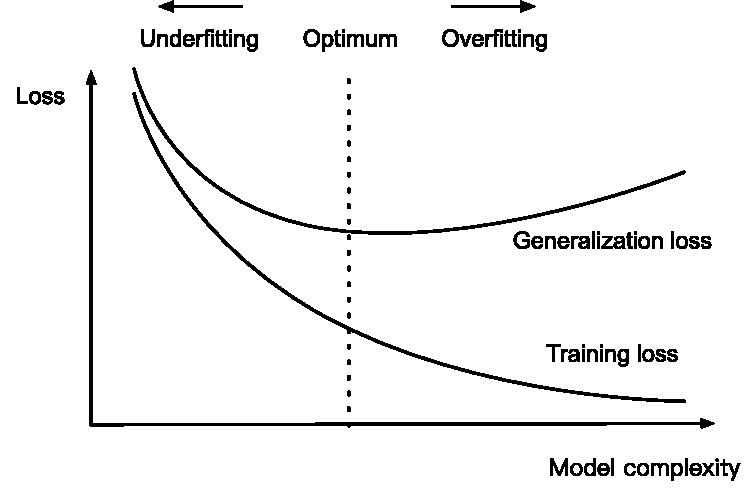
\includegraphics[width = 0.6\linewidth]{capacity-vs-error.pdf}
     \caption{Ảnh hưởng của độ phức tạp của mô hình đến underfitting và overfitting, nguồn: Dive into Deep Learning}
     \label{fig20}
 \end{figure}
 Hình \ref{fig20} minh họa cho hiện tượng quá khớp và dưới khớp!
 \subsubsection{Suy giảm trọng số - Weight decay}
 Câu hỏi đặt ra là một hàm số như thế nào là được coi là phức tạp? Một cách đơn giản để đo độ phức tạp của hàm tuyến tính $f(\textbf{x}) = \textbf{x}^{\text{T}}\textbf{w}$ là chuẩn của vector trọng số, ví dụ $||w||^2$. Do đó ý tưởng là thay vì ta tối thiếu hàm mất mát, ta sẽ tối thiểu hàm mất mát cộng với chuẩn của trọng số. Khi đó chuẩn của nó đóng vai trò như là một thành phần phạt. Quá trình này khá tự động, có thể hình dung như sau: nếu vector trọng số tăng quá lớn thì thuật toán học sẽ tập trung giảm thiểu trọng số của nó thay vì giảm thiểu hàm mất mát!\\\\
 Hàm mất mát sau khi cộng thêm suy giảm trọng số thường có dạng như sau:
 \begin{equation}
     J' = J+\frac{\lambda}{2}||\textbf{w}||^{2}, \lambda>0
     \label{eq49}
 \end{equation}
 Việc dùng chuẩn bình phương có lẽ không cần phải bàn nữa. Ngoài ra, ta cũng cần quan tâm đến chuẩn mà ta sẽ dùng. Thông thường sẽ dùng chuẩn $l_1$ và chuẩn $l_2$. Tùy vào mục đích mà sử dụng, ví dụ như chuẩn $l_2$ nó phạt nặng những thành phần lớn của vector trọng số, điều này khiến thuật toán học thiên vị các mô hình có trọng số được phân bố đồng đều cho một số lượng lớn các đặc trưng. Trong thực tế, điều này có thể giúp giảm ảnh hưởng từ lỗi đo lường của từng biến đơn lẻ. Ngược lại, lượng phạt $l_1$ hướng đến các mô hình mà trọng số chỉ tập trung vào một số lượng nhỏ các đặc trưng, và ta có thể muốn điều này vì một số lí do khác!\\\\
 Trong công thức (\ref{eq49}), ta còn một thành phần đó là $\lambda$, $\lambda$ thể hiện sự ràng buộc của của \textbf{w}, nếu nhỏ thì ràng buộc ít hoặc không bị ràng buộc, còn lớn thì ngược lại. 

 \subsubsection{Dropout}
 Lí thuyết khái quất cổ điển cho rằng: để thu hẹp khoảng cách giữa chất lượng khi huấn luyện và chất lượng khi kiểm tra, ta nên hướng đến một mô hình \textit{đơn giản}. Sự đơn giản này có thể nằm ở số chiều đặc trưng thấp, suy giảm trọng số hướng tới điều này. Ngoài ra, một khái niệm hữu ích khác để biểu diễn sự đơn giản là độ mượt, tức là hàm số không nên quá nhạy cảm với những thay đổi nhỏ ở đầu vào.\\\\
 Vào năm 1995, Christopher Bishop đã chính quy hóa ý tưởng này khi ông chứng minh rằng việc huấn luyện với đầu vào chứa nhiễu tương đương với điều chuẩn Tikhonov (Bishop, 1995). Tức là việc huấn luyện với đầu vào có nhiễu có liên hệ với khả năng kháng nhiễu đầu vào của hàm số. Do đó vào năm 2014, Strivastava et al. (Strivastava et al, 2014) đã đề xuất rằng nên thêm nhiễu vào mỗi tầng của mạng trước khi tính toán trong tầng kế tiếp.\\\\
 Ý tưởng này có tên là \textit{dropout}, hoạt động bằng cách thêm nhiễu khi tính toán các tầng nội bộ trong lan truyền xuôi và nó đã trở thành một kĩ thuật tiêu chuẩn để huấn luyện các mạng neuron. Phương pháp này sẽ \textit{bỏ} (dropout) một số neuron trong quá trình huấn luyện. Tại mỗi vòng lặp huấn luyện, phương pháp dropout tiêu chuẩn sẽ đặt giá trị của một lượng nhất định (thường 50\%) các nút trong mỗi tầng về không trước khi tính toán.\\\\
 Nguyên tắc thêm nhiễu, thêm nhiễu một cách \textit{không thiên lệch} sao cho giá trị kì vọng của mỗi tầng bằng giá trị kì vọng của chính tầng đó trước khi được thêm nhiễu, giả sử rằng các tầng khác được giữ nguyên. \\\\
 Với điều chuẩn dropout tiêu chuẩn, ta khử độ lệch tại mỗi tầng bằng cách chuẩn hóa theo tỉ lệ các nút được giữ lại (chứ không phải các nút bị loại bỏ). Nói cách khác, dropout với \textit{xác suất dropout p} được áp dụng như sau:
 \begin{equation}
     h' = \begin{cases}
         0, \text{ với xác suất $p$} \\
         \frac{h}{1-p}, \text{ khác}
    \label{eq50}
     \end{cases}
 \end{equation}
 Thông thường, \textbf{chúng ta sẽ vô hiệu hóa dropout tại thời điểm kiểm tra}.
 \begin{figure}[ht!]
     \centering
     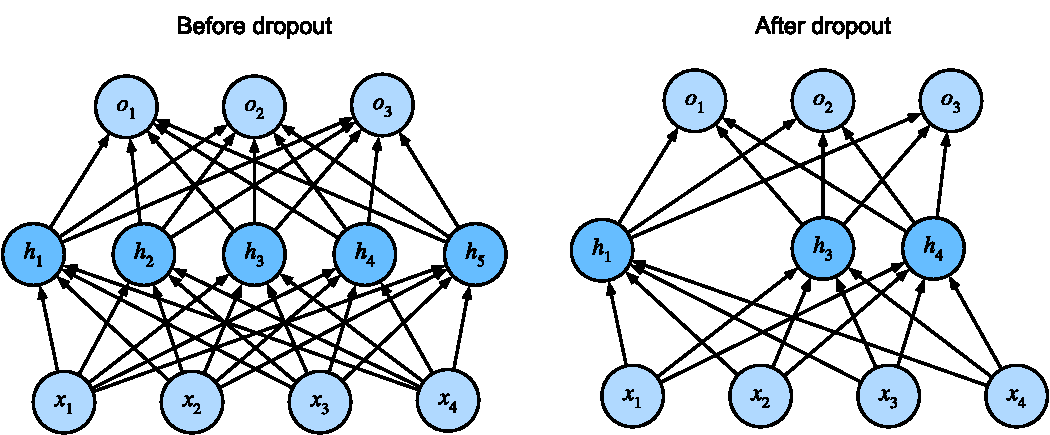
\includegraphics[width = 0.6\linewidth]{dropout2.pdf}
     \caption{MLP before and after dropout, nguồn: Dive into Deep Learning}
     \label{fig21}
 \end{figure}
 \subsection{Autograd và Backpropagation}
 \subsubsection{Computational graph}
 Trước tiên ta cần làm quen với khái niệm \textit{đồ thị tính toán} - Computational graph. \textit{Đồ thị tính toán} là đồ thị có hướng, các nốt ứng với các phép toán hoặc các biến. Đồ thị tính toán giúp chúng ta hình dung được sự phụ thuộc giữa các toán tử và các biến trong quá trình tính toán.
 \begin{figure}[ht!]
     \centering
     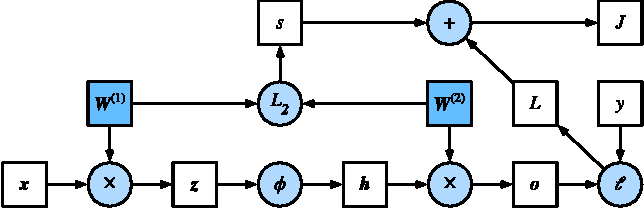
\includegraphics[width = 0.6\linewidth]{forward.pdf}
     \caption{Đồ thị tính toán, nguồn: Dive into Deep Learning}
     \label{fig22}
 \end{figure}
 \subsubsection{Lan truyền xuôi}
 Khái niệm lan truyền xuôi ở đây cũng giống như khái niệm lan truyền xuôi đã đề cập đến ở MLP đa tầng. Tuy nhiên ta sẽ định nghĩa khác một chút, lan truyền xuôi ở đây là quá trình tính toán cũng như lưu trữ các biến trung gian (bao gồm cả đầu ra) của mjng neuron theo thứ tự từ tầng đầu vào đến tầng đầu ra. 
 \subsubsection{Lan truyền ngược}
 Lan truyền ngược là phương pháp tính gradient của các tham số mạng neuron. Phương thức này duyệt qua mạng neuron theo chiều ngược lại từ đầu ra đến đầu vào theo quy tắc chuỗi (chain rule).\\\\
 Lan truyền ngược lưu trữ các biến trung gian (các đạo hàm riêng) cần thiết trong quá trình tính toán gradient theo các tham số.\\\\
 \underline{Nhận xét}: Khi huấn luyện các mô hình học sâu, lan truyền xuôi và ngược phụ thuộc lẫn nhau.
  \begin{figure}[ht!]
     \centering
     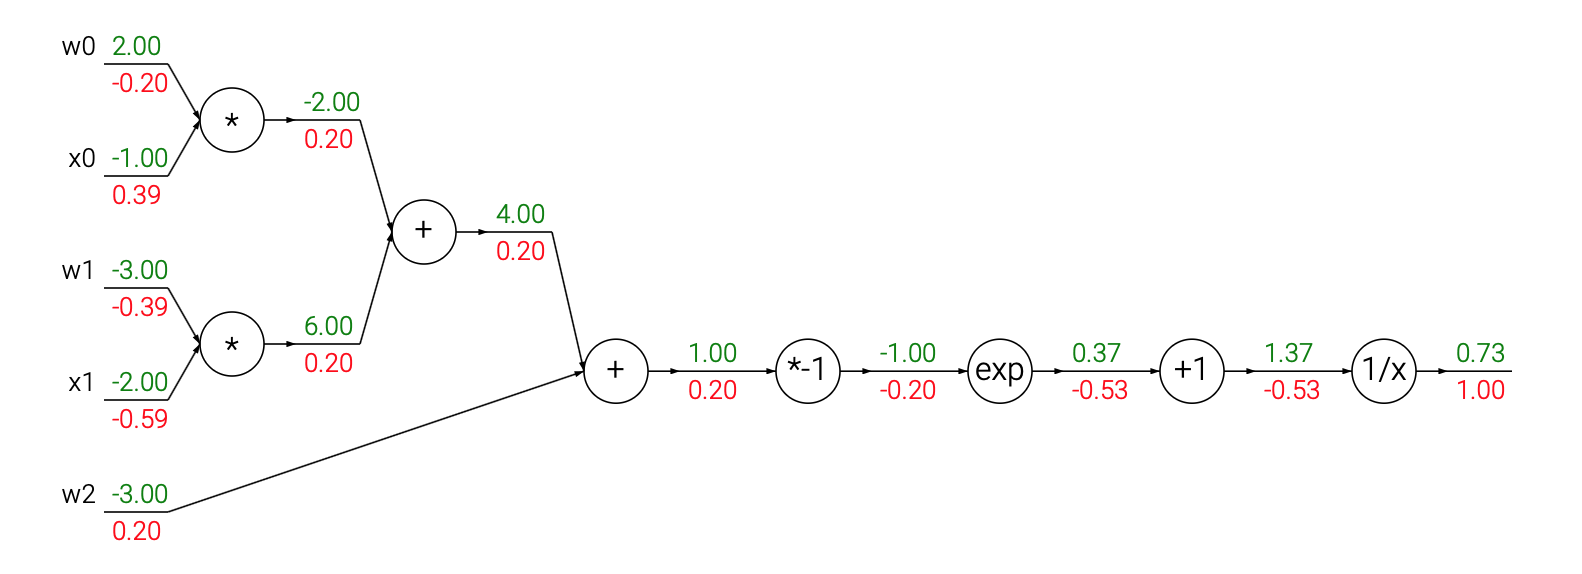
\includegraphics[width = \linewidth]{4.png}
     \caption{Lan truyền xuôi (xanh), lan truyền ngược (đỏ)}
     \label{fig23}
 \end{figure}
 \subsubsection{Autograd}
 Là công cụ tính vi phân tự động dựa trên lan truyền xuôi và lan truyền ngược!
 \section{Mã nguồn}
 Mã nguồn cho bài này có thể tìm thấy ở đây: \\\url{https://github.com/thuantn210823/Computer-Vision-IPSAL-LAB-}
    \newpage
\section{Tài liệu tham khảo}
    \begin{thebibliography}{9}
        \bibitem{slide}
        Truong. PV, Thao. TT Bài giảng , Đại học Bách Khoa Hà Nội.
        \bibitem{slide}
        Tiep. HV \emph{Machine Learning cơ bản}, Nhà xuất bản khoa học và kĩ thuật.
        \bibitem{book}
        Aston Zhang, Zachary C.Lipton, Mu Li, and Alexander J. Smola \emph{Dive into Deep Learning}.
        \bibitem{book}
        Quỳ. TĐ \emph{Giáo trình Xác suất thống kê}, Nhà xuất bản Đại học Bách Khoa Hà Nội.
        \bibitem{website}
        \url{d2l.aivivn.com}
        \bibitem{website}
        \url{machinelearningcoban.com}

    \end{thebibliography}
\end{document}
